\documentclass[11pt,a4paper,oneside]{article}

\usepackage[utf8]{inputenc}
\usepackage[T1]{fontenc}
\usepackage[spanish,es-tabla]{babel}
\usepackage{newtxtext,newtxmath} % Tipo de letra estilo Times compatible con pdfLaTeX
\usepackage[a4paper,left=3cm,right=3cm,top=2.5cm,bottom=2.5cm]{geometry}
\usepackage{setspace}
\setstretch{1.2}
\usepackage{microtype}
\usepackage{amsmath}
\usepackage{graphicx,booktabs,tabularx,array}
\usepackage{float}
\usepackage{xcolor}
\usepackage{tikz}
\usetikzlibrary{arrows.meta,positioning,shapes.geometric}
\usepackage{listings}
\usepackage{csquotes}
\usepackage[backend=biber,style=ieee,citestyle=numeric,sorting=none]{biblatex}
\addbibresource{referencias.bib}
\usepackage{fancyhdr}
\usepackage{lastpage}
\usepackage{xurl}
\usepackage{hyperref}

\definecolor{azulUTEQ}{HTML}{183C60}
\definecolor{grisNota}{HTML}{666666}
\hypersetup{colorlinks=true,linkcolor=azulUTEQ,citecolor=azulUTEQ,urlcolor=azulUTEQ,pdftitle={Práctica experimental U1: sockets TCP, gRPC y Lamport}}
\lstdefinestyle{codigo}{
 basicstyle=\ttfamily\footnotesize,
 breaklines=true,
 frame=single,
 numbers=left,
 numberstyle=\tiny,
 showstringspaces=false,
 tabsize=4,
 captionpos=b
}
\lstset{style=codigo}

\newif\ifmodoBorrador
\modoBorradorfalse
\newcommand{\pendiente}[1]{%
  \par\smallskip\noindent{\color{grisNota}\textbf{[PENDIENTE]} #1}\par\smallskip
}
\pagestyle{fancy}
\fancyhf{}
\fancyhead[L]{\footnotesize GA-SUM-01 / PE-U1}
\fancyhead[R]{\ifmodoBorrador\footnotesize\textcolor{red!70!black}{BORRADOR / NO ENTREGAR}\fi}
\fancyfoot[C]{\thepage\ de \pageref{LastPage}}
\setlength{\headheight}{15pt}
\renewcommand{\headrulewidth}{0.4pt}

\begin{document}
\hypersetup{pageanchor=false}
\begin{titlepage}
\centering
{\Large\textbf{UNIVERSIDAD TÉCNICA ESTATAL DE QUEVEDO}}\\[0.45cm]
{\large Facultad de Ciencias de la Computación}\\[0.15cm]
{\large Carrera de Software}\\[1.35cm]
{\LARGE\bfseries PRÁCTICA EXPERIMENTAL -- UNIDAD 1}\\[0.3cm]
{\Large Comunicación entre procesos mediante sockets TCP y gRPC}\\[0.25cm]
{\large Verificación con relojes lógicos de Lamport}\\[1.3cm]
\begin{tabular}{@{}ll@{}}
\textbf{Asignatura:} & Aplicaciones Distribuidas \\
\textbf{Código de actividad:} & GA-SUM-01 / PE-U1 \\
\textbf{Nivel / paralelo:} & Séptimo nivel / A \\
\textbf{Modalidad:} & Grupal \\
\textbf{Docente:} & Gleiston Cicerón Guerrero Ulloa \\
\textbf{Fecha límite:} & 21 de noviembre de 2026, 23:59 \\
\end{tabular}
\\[1.0cm]
{\large\textbf{Integrantes}}\\[0.25cm]
Calderon Saltos Joseph Alexander \\[0.12cm]
Garcia Sangoquiza Roger Steven \\[0.12cm]
Mera Jumbo Allison Michelle \\[0.12cm]
Zambrano Parraga Luis Mario
\vfill
\textbf{Repositorio público:}\\[0.1cm]
{\scriptsize\href{https://github.com/Yukisan-uwo/GA-SUM-02-PE-U1-Practica-Experimental-Unidad-1}{\nolinkurl{https://github.com/Yukisan-uwo/GA-SUM-02-PE-U1-Practica-Experimental-Unidad-1}}}
\\[0.7cm]
{\small Quevedo, Ecuador -- noviembre de 2026}
\end{titlepage}

\hypersetup{pageanchor=true}
\pagenumbering{roman}
\section*{Resumen}
\addcontentsline{toc}{section}{Resumen}

Esta práctica comparó dos mecanismos de comunicación entre procesos: sockets TCP con mensajes JSON y gRPC con Protocol Buffers. También incorporó relojes lógicos de Lamport para verificar el cumplimiento de sus reglas de ordenamiento en los eventos registrados. Se realizaron un benchmark secuencial y pruebas funcionales con tres nodos. En el benchmark, ejecutado en Windows sobre localhost, se obtuvieron 2000 mediciones de latencia de ida y vuelta (RTT): cinco corridas de 100 solicitudes por mecanismo y tamaño de carga (100 y 10240 bytes), excluyendo el calentamiento. TCP registró una latencia media de 0,122\,ms frente a 0,547\,ms de gRPC con 100 bytes; con 10240 bytes, las medias fueron 0,197 y 0,564\,ms, respectivamente. TCP también alcanzó mayor rendimiento en mensajes por segundo con ambas cargas. Las corridas funcionales de 20 intercambios por mecanismo y cuatro pruebas automatizadas concurrentes de 300 solicitudes por condición completaron los intercambios, sin errores causales reportados por el verificador de Lamport. Las pruebas concurrentes se ejecutaron en Linux y no se mezclaron con las mediciones de Windows. Los resultados respaldan la hipótesis inicial en el entorno evaluado, pero no permiten generalizar la superioridad de TCP ni demostrar tolerancia ante fallos no ensayados.

\par\smallskip
\noindent\textbf{Palabras clave:}
sistemas distribuidos, sockets TCP, gRPC,
relojes de Lamport, latencia.

\vspace{0.6cm}

\section*{Abstract}
\addcontentsline{toc}{section}{Abstract}

This study compared two interprocess communication mechanisms: TCP sockets with JSON messages and gRPC with Protocol Buffers. It also incorporated Lamport logical clocks to verify compliance with their ordering rules in the recorded events. A sequential benchmark and functional tests involving three nodes were conducted. In the benchmark, performed on Windows over localhost, 2000 round-trip time (RTT) measurements were collected: five runs of 100 requests for each combination of communication mechanism and payload size (100 and 10240 bytes), excluding warm-up runs. TCP achieved a mean latency of 0.122\,ms compared with 0.547\,ms for gRPC with 100-byte messages; with 10240 bytes, the means were 0.197 and 0.564\,ms, respectively. TCP also achieved higher throughput, measured in messages per second, for both payload sizes. The functional runs of 20 exchanges per mechanism and four automated concurrent tests of 300 requests per condition completed the exchanges, with no causal errors reported by the Lamport verifier. The concurrent tests were conducted on Linux and were not combined with the Windows measurements. The results support the initial hypothesis under the evaluated conditions, but do not establish that TCP is universally superior or demonstrate tolerance to failures that were not tested.

\par\smallskip
\noindent\textbf{Keywords:}
distributed systems, TCP sockets, gRPC,
Lamport clocks, latency.
\clearpage

\tableofcontents
\clearpage
\pagenumbering{arabic}

\section{Objetivos e hipótesis}

\subsection{Objetivo general}

Comparar el desempeño de la comunicación mediante sockets
TCP y gRPC con Protocol Buffers en un entorno distribuido
de tres nodos, a partir de mediciones de latencia y
rendimiento, y comprobar el orden de los eventos mediante
relojes lógicos de Lamport.

\subsection{Objetivos específicos}

\begin{enumerate}

    \item Configurar tres nodos independientes en
    localhost, identificados como nodo-A, nodo-B y
    nodo-C, y verificar el intercambio de mensajes
    mediante sockets TCP y gRPC.

    \item Registrar veinte intercambios por mecanismo
    con sus respectivas marcas de tiempo de Lamport,
    de manera que sea posible analizar el orden
    de envío y recepción de los mensajes.

    \item Medir la latencia de ida y vuelta (RTT)
    con cargas útiles de 100 y 10240 bytes,
    utilizando cinco corridas de cien envíos
    por condición y descartando una corrida
    previa de calentamiento.

    \item Comparar la latencia media, mediana,
    desviación estándar, percentil 95 y rendimiento
    de ambos mecanismos a partir de los registros
    obtenidos durante las pruebas.

    \item Evaluar la comunicación con tres clientes
    concurrentes y verificar las relaciones de
    causalidad observables en los registros de
    eventos.

\end{enumerate}

\subsection{Hipótesis previa a la experimentación}

Se plantea que la implementación con sockets TCP
presentará una latencia media de ida y vuelta menor
que gRPC en las pruebas realizadas sobre localhost,
tanto para mensajes de 100 bytes como de 10240 bytes.

Esta expectativa se relaciona con las características
de las implementaciones desarrolladas. En TCP, el
equipo construyó directamente el intercambio de
solicitudes y respuestas mediante mensajes JSON,
aprovechando el servicio de transporte fiable y
orientado a conexión que proporciona el protocolo
\cite{eddy2022tcp}. En cambio, la implementación
gRPC utiliza llamadas a procedimientos remotos,
mensajes definidos con Protocol Buffers y HTTP/2.
El estudio de Niswar et al. \cite{niswar2024grpc}
analiza el rendimiento de gRPC frente a otras
alternativas de comunicación entre microservicios,
lo que refuerza la necesidad de evaluar estos
mecanismos bajo condiciones experimentales
definidas.

La hipótesis no supone que TCP sea más rápido en
cualquier entorno. Su evaluación se limitará a las
implementaciones del equipo y a las condiciones
establecidas para esta práctica. Se considerará
respaldada cuando la latencia media de TCP sea
inferior a la de gRPC en ambos tamaños de mensaje.
Las diferencias observadas se examinarán junto
con la dispersión y el percentil 95 para evitar
que la comparación dependa únicamente del promedio.


\section{Fundamentación teórica de la Unidad 1}
\subsection{Sistemas distribuidos y características fundamentales}

Un sistema distribuido está formado por varios elementos de cómputo autónomos que se comunican por una red y colaboran para ofrecer servicios. Aunque los procesos y recursos estén repartidos entre varios equipos, el sistema busca que el usuario pueda utilizar sus servicios de manera coherente. Esa distribución permite compartir recursos y dividir tareas, pero también introduce latencias, comunicación entre procesos y fallos que pueden afectar solo a una parte del sistema \cite{vanSteenTanenbaum2023}.

Cada nodo ejecuta sus propios procesos y mantiene su estado local. Por eso, los nodos deben intercambiar mensajes para coordinar operaciones; no pueden asumir que todos observan los eventos al mismo tiempo ni que una demora significa necesariamente que otro nodo dejó de funcionar. La coordinación, la concurrencia y la detección de fallos son parte del diseño del sistema distribuido \cite{vanSteenTanenbaum2023}.

\subsection{Sistemas centralizados, paralelos y distribuidos}

En un sistema centralizado, el procesamiento y la administración principal de los recursos se concentran en un equipo o servicio. Los clientes envían solicitudes a ese punto central. Su operación es más sencilla de organizar, aunque ese punto puede convertirse en un límite de capacidad o en una causa de interrupción si falla.

Un sistema paralelo divide una tarea para ejecutar varias partes al mismo tiempo. El paralelismo describe cómo se organiza el procesamiento; puede ocurrir dentro de una computadora o entre varias. En un sistema distribuido, en cambio, los nodos son unidades independientes que se comunican mediante una red. Por ello, un sistema puede ser distribuido y también aprovechar el paralelismo \cite{vanSteenTanenbaum2023}.

En esta práctica, los procesos se identifican como \texttt{nodo-A}, \texttt{nodo-B} y \texttt{nodo-C}. Se ejecutan en \texttt{localhost}, cada uno con un puerto definido. El escenario permite estudiar el intercambio de mensajes entre procesos, aunque no equivale a desplegar los nodos en máquinas físicas distintas.

\subsection{Transparencias ANSA}

Las transparencias buscan ocultar ciertos detalles de la distribución a quienes usan el sistema. El prototipo no las ofrece todas; algunas se observan de forma parcial y otras no están implementadas \cite{vanSteenTanenbaum2023}.

\begin{description}
    \item[Acceso — parcial.] El benchmark utiliza una interfaz común para enviar mensajes con TCP y gRPC. Sin embargo, todavía se debe escoger el cliente correspondiente a cada mecanismo y cada uno usa una representación distinta del mensaje.

    \item[Ubicación — no ofrecida.] Los nodos se identifican mediante nombres, direcciones y puertos. Para conectar el cliente se indica explícitamente el destino, por ejemplo, \texttt{127.0.0.1:5001}.

    \item[Migración — no ofrecida.] El prototipo no traslada procesos o recursos de un nodo a otro mientras mantiene su acceso.

    \item[Reubicación — no ofrecida.] Tampoco mueve un servicio durante una operación activa de forma que el cliente no lo note.

    \item[Replicación — no ofrecida.] La existencia de tres procesos no significa que haya réplicas. En la práctica, los nodos no mantienen copias sincronizadas de un mismo conjunto de datos.

    \item[Concurrencia — parcial.] El servidor TCP crea un hilo por conexión. Las corridas concurrentes automatizadas documentadas en \texttt{data/concurrencia/} usaron tres nodos y procesaron 300 solicitudes totales por condición (100 por nodo), con TCP y gRPC y cargas de 100 y 10240 bytes. Los verificadores no reportaron errores causales. Esto evidencia operación concurrente bajo esas condiciones, pero no demuestra transparencia completa de concurrencia ni manejo de datos de negocio compartidos. La procedencia de las corridas se detalla en \texttt{data/concurrencia/PROCEDENCIA.md}; no se presentan como pruebas personales realizadas en el equipo Windows.

    \item[Fallos — no ofrecida.] Si el servidor no responde o la conexión falla, el cliente recibe el error y lo registra. El prototipo no oculta la interrupción mediante una réplica o una recuperación automática.

    \item[Persistencia — no ofrecida como transparencia.] El programa guarda registros de eventos y latencias en archivos CSV locales. Ese registro no constituye una capa de almacenamiento que oculte al cliente dónde o cómo se conserva la información.
\end{description}

\subsection{Teorema CAP: conceptos y alcance}

CAP describe un compromiso que aparece cuando una partición de red impide que algunos nodos se comuniquen. La consistencia exige que las operaciones se comporten como si se hubieran aplicado en un orden común; la disponibilidad exige que cada solicitud dirigida a un nodo que sigue activo reciba una respuesta. La tolerancia a particiones se refiere a que el sistema continúe operando ante esa pérdida de comunicación.

Cuando existe una partición, un sistema no puede garantizar simultáneamente consistencia y disponibilidad para todas las solicitudes. Debe decidir cómo responder mientras dure el problema: puede rechazar o demorar ciertas operaciones para conservar consistencia, o responder aunque algunos datos todavía no estén actualizados. CAP trata de este escenario de partición; no significa que cualquier sistema simplemente escoja dos propiedades en toda situación \cite{lee2023cap,vanSteenTanenbaum2023}.

La clasificación de un sistema real requiere analizar cómo responde ante una partición. La aplicación de CAP al prototipo y sus límites se desarrollará junto con los resultados de la práctica.
% Autoría principal: Mera. Revisar en equipo.
\subsection{Sockets TCP y UDP}
\pendiente{Describir TCP y UDP a nivel conceptual. La implementación evaluada por el SGA corresponde a sockets TCP, no se exige construir UDP.}

\subsection{RPC, gRPC y Protocol Buffers}
\pendiente{Explicar el modelo solicitud-respuesta, contratos .proto, serialización binaria y diferencias con mensajes JSON.}

\subsection{RMI en Java}
\pendiente{Presentar RMI como antecedente/comparación teórica de RPC, tal como pide la guía.}

\subsection{Diagramas de secuencia y expectativas de rendimiento}
\pendiente{Incorporar o referenciar diagramas propios y formular expectativas justificadas, sin reportar resultados anticipados.}

% Desarrollo con asistencia de IA; pendiente de revisión del integrante responsable.
\subsection{Tiempo físico, causalidad y concurrencia}
La hora del sistema permite fechar un registro, pero no basta para determinar
qué evento causó otro: los relojes físicos pueden diferir y el orden de llegada
depende de la red y de la planificación de procesos. Los relojes lógicos
representan restricciones de orden, no segundos transcurridos
\cite{vanSteenTanenbaum2023}.

La relación de precedencia causal, escrita $a\rightarrow b$, se define por:
\begin{enumerate}
  \item El orden de los eventos dentro de un mismo proceso.
  \item El envío de un mensaje antes de su recepción.
  \item La transitividad: si $a\rightarrow b$ y $b\rightarrow c$, entonces
  $a\rightarrow c$.
\end{enumerate}
Dos eventos son concurrentes cuando no se cumple ninguna de las relaciones
$a\rightarrow b$ ni $b\rightarrow a$. Esta concurrencia es causal: no exige
que ambos eventos ocurran en el mismo instante físico.

\subsection{Reglas del reloj de Lamport}
Cada nodo $i$ mantiene un contador $L_i$, inicialmente cero. Antes de registrar
un evento local o enviar un mensaje, realiza:
\begin{equation}
L_i \leftarrow L_i+1.
\label{eq:lamport-envio}
\end{equation}
El mensaje transporta el contador resultante. Si se recibe una marca $t$, la
actualización es:
\begin{equation}
L_i \leftarrow \max(L_i,t)+1.
\label{eq:lamport-recepcion}
\end{equation}
La recepción y el envío de su acuse son eventos distintos; por ello, el acuse
requiere otro incremento. Estas reglas garantizan la condición del reloj:
\begin{equation}
a\rightarrow b \;\Longrightarrow\; L(a)<L(b).
\end{equation}
El recíproco es falso: $L(a)<L(b)$ no demuestra que exista una cadena causal
entre ambos. Tampoco una diferencia de cinco unidades representa cinco
mensajes ni una duración física de cinco unidades de tiempo
\cite{vanSteenTanenbaum2023}.

Dos eventos de nodos distintos con la misma marca no pueden estar relacionados
por precedencia causal si se cumplen las reglas anteriores. Sin embargo, una
marca escalar no permite decidir la concurrencia para todos los pares de eventos:
también puede haber eventos concurrentes con marcas diferentes. Ordenar por
la pareja $(L,\mathrm{id\ del\ nodo})$ permite desempatar de forma determinista,
pero ese orden total no convierte los eventos en causalmente relacionados.

\subsection{Comparación con relojes vectoriales}
En un sistema de tres nodos, un reloj vectorial mantiene tres componentes,
una por nodo. En un evento local o envío se incrementa la componente propia;
al recibir se combina el vector local y el recibido mediante máximos por
componente y después se incrementa la componente del receptor.
Para dos vectores $V(a)$ y $V(b)$, se escribe $V(a)<V(b)$ si todas las
componentes del primero son menores o iguales y al menos una es estrictamente
menor. Bajo el modelo habitual de procesos y mensajes, esta comparación
representa la precedencia causal; vectores incomparables identifican
concurrencia \cite{vanSteenTanenbaum2023}.

El costo es mantener y transmitir información proporcional al número de nodos,
frente a un contador escalar en Lamport. Los relojes vectoriales se presentan
como comparación conceptual; no forman parte del módulo implementado.

\subsection{Ejemplo didáctico, no experimental}
Supóngase que A y C, con contadores inicialmente en cero, envían sus primeros
mensajes a B sin haber intercambiado información entre sí. Ambos envíos llevan
marca 1 y son concurrentes. Si B recibe primero el mensaje de A, actualiza su
contador a 2; al enviar el acuse lo incrementa a 3. A recibe ese acuse y pasa
a $\max(1,3)+1=4$. Si luego B recibe el mensaje inicial de C, con marca 1,
su contador pasa a $\max(3,1)+1=4$.

En este ejemplo, el envío de A precede causalmente a su recepción en B,
con $1<2$. Los primeros envíos de A y C tienen la misma marca sin relación
causal entre ellos. Los números anteriores ilustran las reglas; no son
mediciones ni sustituyen la comprobación sobre los CSV de la práctica.

% Autoría principal: Mario Zambrano.

\subsection{Clasificación de fallos}

En un sistema distribuido, los componentes pueden
presentar fallos de distintas formas. Un servidor
puede dejar de funcionar, perder una comunicación
o responder fuera del tiempo esperado. Por eso,
antes de establecer una solución, es importante
identificar qué tipo de fallo se quiere tratar.
Nogueira y Coelho \cite{nogueira2026fault}
explican que las técnicas de recuperación dependen
del modelo de fallos considerado.

Entre los principales tipos se encuentran:

\begin{itemize}

    \item \textbf{Fallo por caída (\textit{crash}):}
    ocurre cuando un proceso deja de ejecutarse
    y ya no responde a las solicitudes. En nuestra
    práctica, una situación de este tipo sería
    detener el servidor del nodo-B mientras otro
    nodo intenta comunicarse con él.

    \item \textbf{Fallo por omisión:}
    se presenta cuando un proceso no realiza un
    envío o una recepción que debía efectuar.
    Para el cliente, uno de los posibles síntomas
    es no recibir la respuesta esperada, aunque
    esto no permite determinar por sí solo la
    causa del problema.

    \item \textbf{Fallo de temporización:}
    aparece cuando una operación se completa
    fuera del intervalo de tiempo establecido.
    La respuesta puede ser correcta, pero llegar
    demasiado tarde para resultar útil.

    \item \textbf{Fallo bizantino:}
    se produce cuando un nodo presenta un
    comportamiento arbitrario. Por ejemplo,
    podría enviar información contradictoria
    a distintos participantes sin dejar de
    funcionar.
\end{itemize}

Los fallos por caída, omisión y temporización
forman parte de los modelos que Nogueira y
Coelho \cite{nogueira2026fault} distinguen
en su estudio sobre tolerancia a fallos.
Por su parte, Zhong et al.
\cite{zhong2023byzantine} explican el
problema de los nodos bizantinos al
analizar algoritmos que deben alcanzar
consenso incluso cuando existen
participantes defectuosos.

Nuestro prototipo permite observar algunos
errores de comunicación, pero no implementa
consenso bizantino ni mecanismos para
tolerar cualquier tipo de fallo.

\subsection{Detección, recuperación y fiabilidad}

Cuando un cliente no recibe una respuesta,
no siempre es posible saber qué ocurrió.
El servidor pudo detenerse, la comunicación
pudo interrumpirse o la solicitud pudo
tardar más de lo esperado. Duarte et al.
\cite{duarte2023detectors} explican que,
en los sistemas asíncronos, resulta difícil
distinguir entre un proceso que ha fallado
y otro que simplemente responde con lentitud.

Una forma de controlar estas situaciones es
establecer tiempos de espera. En nuestra
implementación, los clientes TCP y gRPC
utilizan un límite de dos segundos.
El cliente TCP captura excepciones
relacionadas con la conexión y la lectura
de mensajes, mientras que gRPC permite
identificar errores producidos durante
las llamadas remotas.

Estos errores pueden registrarse en los
archivos de latencia, lo que permite
separar las solicitudes correctas de
aquellas que terminaron con problemas.
Sin embargo, identificar un error no
significa que el servicio se haya
recuperado.

Entre las técnicas de recuperación se
encuentran los reintentos, el reinicio
de componentes y el uso de réplicas.
Nogueira y Coelho \cite{nogueira2026fault}
distinguen la recuperación de un servicio
de la recuperación de su estado, ya que
reiniciar un proceso no garantiza que
se conserven los datos o mensajes
pendientes.

En el trabajo de Marletta et al.
\cite{marletta2024robustness} se presenta
una solución que modifica llamadas remotas
en aplicaciones Java e incorpora políticas
de reintentos. Los autores muestran una
configuración con esperas progresivas y
un número máximo de intentos para
controlar fallos temporales.

En nuestro caso no se implementó una
política propia de reintentos automáticos
ni un mecanismo de recuperación mediante
réplicas. Los clientes pueden detectar y
registrar determinados errores, pero
todavía no cuentan con una solución que
garantice la continuidad del servicio
cuando un nodo deja de funcionar.

\subsection{Seguridad: JWT y OAuth 2.0}

La seguridad de un sistema distribuido
no depende únicamente de que los mensajes
lleguen correctamente. También es necesario
comprobar quién solicita una operación
y si tiene permiso para realizarla.

La autenticación permite comprobar la
identidad de un usuario o proceso,
mientras que la autorización determina
qué recursos puede utilizar. Bucko et al.
\cite{bucko2023jwt} explican esta
diferencia y presentan una aplicación
web que utiliza JWT como parte de su
mecanismo de control de acceso.

JSON Web Token (JWT) permite representar
información mediante un token que contiene
declaraciones sobre su portador. En las
implementaciones con firma, esta puede
utilizarse para comprobar que el contenido
no fue modificado. El token también puede
contener datos como el identificador del
usuario o su tiempo de expiración.
Bucko et al. \cite{bucko2023jwt}
describen su utilización en el proceso
de autenticación y autorización de
una aplicación web.

OAuth 2.0 cumple una función diferente.
Es un marco de autorización que permite
conceder acceso limitado a determinados
recursos sin entregar directamente las
credenciales del usuario a la aplicación
que solicita el acceso.

Almeida y Canedo
\cite{almeida2022authmicroservices}
identifican OAuth 2.0 y JWT entre los
mecanismos utilizados para proteger
aplicaciones basadas en microservicios.
También explican que ambos pueden
emplearse conjuntamente, aunque uno
establece un mecanismo de autorización
y el otro define un formato de token.

La seguridad de los tokens requiere
validaciones adecuadas y protección
durante su transmisión. Por ejemplo,
una firma digital no reemplaza el
cifrado del canal de comunicación.

En nuestra práctica, los mensajes TCP
se intercambian mediante JSON y las
llamadas gRPC utilizan Protocol Buffers.
No se implementaron JWT, OAuth 2.0
ni un mecanismo de autenticación de
usuarios. Además, las conexiones se
realizaron en localhost sin configurar
TLS.

Por tanto, estas tecnologías se estudian
como alternativas para proteger una
aplicación distribuida que deba gestionar
usuarios, permisos y acceso a servicios,
pero no forman parte de las funciones
implementadas en esta práctica.

\subsection{CAP y ejemplos de aplicaciones reales}

El teorema CAP explica una limitación
de los sistemas distribuidos que
mantienen información compartida entre
varios nodos. Sus tres propiedades son
consistencia, disponibilidad y tolerancia
a particiones de red.

La consistencia está relacionada con
mantener una visión coherente de los
datos compartidos. La disponibilidad
se refiere a la capacidad de responder
a las solicitudes, mientras que una
partición ocurre cuando se interrumpe
la comunicación entre grupos de nodos.

Durante una partición, un sistema no
puede garantizar al mismo tiempo
consistencia fuerte y disponibilidad
para todas las solicitudes. Lee et al.
\cite{lee2023cap} estudian esta
relación y muestran cómo los requisitos
de consistencia y disponibilidad
también se relacionan con la latencia
de comunicación.

Este problema puede observarse, por
ejemplo, en una aplicación que mantiene
copias del inventario de una tienda
en distintos servidores. Si estos
pierden la comunicación, aceptar
nuevas compras sin confirmar las
existencias podría ocasionar datos
inconsistentes. Una alternativa
sería detener temporalmente ciertas
operaciones hasta recuperar la
comunicación.

En cambio, una aplicación de
publicaciones podría permitir que
los usuarios continúen registrando
contenido durante una interrupción.
Para hacerlo tendría que aceptar
diferencias temporales entre las
copias y resolverlas posteriormente.

Los casos anteriores son ejemplos
hipotéticos. Su finalidad es mostrar
que las decisiones sobre consistencia
y disponibilidad dependen de las
necesidades de cada aplicación.

Es importante aclarar que CAP no
determina si conviene utilizar sockets
TCP o gRPC. Ambos son mecanismos de
comunicación, mientras que CAP trata
sobre las garantías de un sistema que
mantiene datos distribuidos.

En nuestra práctica se compararon
latencias y rendimiento de TCP y gRPC,
y se incorporaron relojes de Lamport
para registrar el orden de los eventos.
No se implementó una base de datos
replicada ni se evaluaron formalmente
las propiedades del teorema CAP.
Por esta razón, su aplicación en
el informe es conceptual.


\section{Arquitectura del sistema distribuido}
% Autoría principal: Roger; arquitectura revisada con todos.
\subsection{Diseño de los tres nodos}
\pendiente{Actualizar el diagrama de FORM-TL-01 con nodo-A, nodo-B, nodo-C y puertos 5000, 5001, 5002, indicando qué proceso actúa como servidor y cliente. No presentar una arquitectura propuesta como ejecutada.}

\subsection{Diagrama de arquitectura (TikZ)}
% Crear figures/arquitectura_tikz.tex desde el diagrama real FORM-TL-01.
\IfFileExists{figures/arquitectura_tikz.tex}{%
 \begin{figure}[htbp]\centering\begingroup
\shorthandoff{<>}
\begin{tikzpicture}[
  node distance=2cm and 3cm,
  every node/.style={align=center},
  box/.style={draw,rounded corners,text width=4cm,minimum height=1.6cm},
  >=Stealth]
\node[box] (a) {nodo-A:5000\\Servidor + cliente\\Reloj A + registro A};
\node[box,right=of a] (b) {nodo-B:5001\\Servidor + cliente\\Reloj B + registro B};
\node[box,below=of a,xshift=3.5cm] (c) {nodo-C:5002\\Servidor + cliente\\Reloj C + registro C};
\draw[->,thick] (a) -- node[above] {solicitudes} (b);
\draw[->,thick] (b) -- node[right] {solicitudes} (c);
\draw[->,thick] (c) -- node[left] {solicitudes} (a);
\end{tikzpicture}
\endgroup

 \caption{Arquitectura validada de los tres nodos (diagrama del equipo).}\label{fig:arquitectura}\end{figure}
}{\pendiente{Crear docs/figures/arquitectura\_tikz.tex con el diagrama real basado en FORM-TL-01.}}

\subsection{Modelo de mensajes y flujo de comunicación}
\pendiente{Mostrar estructura JSON {\ttfamily\{sender, timestamp, message\}}, su equivalente Protocol Buffers, direcciones de mensajes y correlación de solicitud/respuesta.}

\subsection{Ejecución y decisiones de despliegue}
\pendiente{Explicar si se ejecutan procesos en localhost o contenedores Docker, y cómo se evitan conflictos de puertos cuando se comparan los dos mecanismos.}


\section{Implementación}
% Autoría principal: Joseph; respaldar con archivos REALES.

\subsection{Implementación con sockets TCP}

En la prueba local, \texttt{nodo-A} envía solicitudes a \texttt{nodo-B}, que escucha en \texttt{127.0.0.1:5001}. El cliente abre una conexión TCP y la reutiliza para los mensajes de la corrida. Cada solicitud contiene \texttt{sender}, \texttt{timestamp} y \texttt{message} en un objeto JSON codificado en UTF-8. Como TCP entrega un flujo de bytes, el programa añade un salto de línea para separar los mensajes. El servidor lee cada línea, valida sus campos y responde con \texttt{receiver}, \texttt{timestamp} y \texttt{ok} \cite{eddy2022tcp,bray2017json}.

El cliente mide el tiempo desde que empieza a escribir la solicitud hasta que recibe el acuse. El código registra los eventos de cada nodo en archivos CSV y añade las latencias a \texttt{data/latencias\_tcp.csv}. También usa un límite de espera de dos segundos. La prueba que tenemos documentada es entre \texttt{nodo-A} y \texttt{nodo-B}; no la describimos como una prueba de los tres nodos.

\subsubsection{Fragmento representativo de código TCP}

El cliente prepara la solicitud, registra el envío y espera el acuse por la misma conexión:

\begin{lstlisting}[language=Python,caption={Envío de una solicitud TCP y recepción del acuse}]
request = {"sender": sender, "timestamp": self.clock.tick(), "message": message}
append_event(sender, "envio_solicitud", request["timestamp"], message_id, sender, destination)
started = time.perf_counter()
self.writer.write(json.dumps(request, ensure_ascii=False, separators=(",", ":")) + "\n")
self.writer.flush()
response = receive_json_line(self.reader)
\end{lstlisting}

\subsubsection{Ejecución de 20 intercambios y registro de eventos}
\pendiente{Agregar el CSV generado por la corrida y describir los 20 intercambios con sus datos observados.}
% Autoría principal: Mera; respaldar con archivos REALES.
\subsection{Implementación con gRPC y Protocol Buffers}

En la versión gRPC, cada nodo publica un servicio remoto y el cliente invoca un método de ese servicio como si fuera una función local. El intercambio es el mismo que en TCP: el emisor envía \texttt{sender}, \texttt{timestamp} y \texttt{message}, y el receptor responde con \texttt{receiver}, \texttt{timestamp} y \texttt{ok}. La diferencia está en quién construye y lee los mensajes. En TCP el programa arma el JSON, lo delimita con un salto de línea y valida cada campo; en gRPC esa tarea la hacen las clases generadas a partir del contrato \texttt{.proto}, que serializan los datos en formato binario y los envían sobre HTTP/2 \cite{niswar2024grpc,sliwa2021grpc}.

El código está en \texttt{src/grpc/}:
\begin{itemize}
	\item \texttt{messaging.proto}: contrato del servicio y de los mensajes.
	\item \texttt{messaging\_pb2.py} y \texttt{messaging\_pb2\_grpc.py}: código generado con \texttt{grpcio-tools}; no se edita a mano.
	\item \texttt{server\_grpc.py}: servidor de un nodo (\texttt{nodo-A}, \texttt{nodo-B} o \texttt{nodo-C}, en los puertos 5000, 5001 y 5002).
	\item \texttt{client\_grpc.py}: cliente con la misma interfaz que el cliente TCP (\texttt{conectar}, \texttt{enviar}, \texttt{cerrar}).
	\item \texttt{registro\_grpc.py}: escritura de eventos y latencias en CSV, con las mismas columnas que el registro TCP.
\end{itemize}
El reloj lógico no se implementó por separado: tanto el servidor como el cliente usan la clase \texttt{LamportClock} de \texttt{src/common/lamport.py}, la misma que usa TCP y que se describe en la implementación del reloj de Lamport.

\subsubsection{Contrato de servicio (.proto)}

El contrato define un servicio con un único procedimiento remoto, \texttt{EnviarMensaje}, que recibe un \texttt{Request} y devuelve un \texttt{Response}. Los nombres del servicio y de los mensajes siguen la guía de la práctica, y los campos son los mismos que se acordaron para el JSON de TCP.

\begin{lstlisting}[caption={Contrato \texttt{src/grpc/messaging.proto}}]
	syntax = "proto3";
	
	package messaging;
	
	service MessagingService {
		rpc EnviarMensaje (Request) returns (Response);
	}
	
	message Request {
		string sender = 1;
		int64 timestamp = 2;
		string message = 3;
	}
	
	message Response {
		string receiver = 1;
		int64 timestamp = 2;
		bool ok = 3;
	}
\end{lstlisting}

Los números \texttt{= 1}, \texttt{= 2} y \texttt{= 3} no son valores, sino las etiquetas con las que cada campo viaja en el mensaje binario; por eso el nombre del campo no se transmite y las etiquetas no deben cambiarse una vez publicado el contrato. El reloj se declaró como \texttt{int64} porque es un contador entero que solo crece. El código Python se generó desde \texttt{src/grpc/} con el comando indicado en la guía:

\begin{lstlisting}[language=bash,caption={Generación del código a partir del contrato}]
	python -m grpc_tools.protoc -I. --python_out=. --grpc_python_out=. messaging.proto
\end{lstlisting}

Para ver el efecto de la codificación binaria, se serializó el mismo contenido con Protocol Buffers y con el JSON compacto que usa el cliente TCP. La tabla~\ref{tab:tamanos-serializados} muestra el tamaño de cada mensaje sin contar el salto de línea que TCP añade como delimitador ni las cabeceras de HTTP/2. La diferencia es de 33 o 34 bytes por solicitud: pesa en mensajes cortos, pero en uno de 10\,KB representa menos del 0,4\,\%.

\par\medskip
\noindent\begin{minipage}{\linewidth}
	\centering
	\makeatletter\def\@captype{table}\makeatother
	\caption{Tamaño serializado de una solicitud y un acuse (bytes)}
	\label{tab:tamanos-serializados}
	\begin{tabular}{@{}lrr@{}}
		\toprule
		Contenido & Protocol Buffers & JSON compacto \\
		\midrule
		Solicitud con \texttt{message = "hola"} & 16 & 50 \\
		Solicitud con carga de 100 bytes & 112 & 146 \\
		Solicitud con carga de 10\,240 bytes & 10\,253 & 10\,286 \\
		Acuse (\texttt{receiver}, \texttt{timestamp = 79}, \texttt{ok}) & 12 & 46 \\
		\bottomrule
	\end{tabular}
\end{minipage}
\par\medskip

\subsubsection{Servidor}

El servidor crea un \texttt{grpc.server} con un grupo de diez hilos, registra el servicio y escucha en \texttt{127.0.0.1} en el puerto de su nodo. Se usa la dirección IPv4 en lugar de \texttt{localhost} para que Windows no intente primero IPv6, lo que añadiría retrasos a las mediciones. Cuando llega una solicitud, el método \texttt{EnviarMensaje} aplica dos eventos de Lamport: la recepción y el envío del acuse.

\begin{lstlisting}[language=Python,caption={Atención de una solicitud en \texttt{server\_grpc.py}}]
	def EnviarMensaje(self, request, context):
	try:
	ts_recepcion = self.reloj.receive(request.timestamp)
	except (TypeError, ValueError) as error:
	context.abort(grpc.StatusCode.INVALID_ARGUMENT, str(error))
	id_mensaje = self._siguiente_id(context.peer(), request.sender)
	# ... registro de recepcion_solicitud ...
	ts_acuse = self.reloj.tick()
	# ... registro de envio_acuse ...
	return messaging_pb2.Response(receiver=self.nombre, timestamp=ts_acuse, ok=True)
\end{lstlisting}

Al recibir se aplica $\max(\text{local}, \text{recibido}) + 1$. Responder con el acuse es un evento nuevo, por lo que se incrementa el reloj una vez más y ese valor es el que viaja en el \texttt{Response}; así se comporta también el servidor TCP. El identificador del mensaje se calcula por conexión (\texttt{context.peer()}) y por emisor, con el formato \texttt{nodo-A-000001}, para que coincida con el que genera el cliente y se pueda emparejar cada envío con su recepción en la verificación de Lamport. La opción \texttt{--silencioso} desactiva la impresión en consola y el registro de eventos, de modo que en las mediciones no se cuente el tiempo de escribir en pantalla o en disco.

\subsubsection{Cliente y medición de la latencia}

El cliente abre un solo canal en \texttt{conectar} y lo reutiliza para todos los envíos de la corrida. Antes de devolver el control espera a que el canal esté listo (\texttt{grpc.channel\_ready\_future}), para que el establecimiento de la conexión no quede dentro de la latencia del primer mensaje. El método \texttt{enviar} recibe los mismos parámetros que el de \texttt{ClienteTCP}, lo que permite que \texttt{analysis/benchmark.py} use cualquiera de los dos clientes sin cambiar el procedimiento de medición.

\begin{lstlisting}[language=Python,caption={Envío y medición del RTT en \texttt{client\_grpc.py}}]
	ts_envio = self.clock.send()
	# ... registro de envio_solicitud (fuera del tiempo medido) ...
	solicitud = messaging_pb2.Request(sender=sender, timestamp=ts_envio, message=message)
	inicio = time.perf_counter()
	acuse = self.stub.EnviarMensaje(solicitud, timeout=self.timeout)
	latencia_ms = (time.perf_counter() - inicio) * 1000
	ts_recepcion = self.clock.receive(acuse.timestamp)
\end{lstlisting}

El tiempo medido comprende la serialización de la solicitud, el viaje de ida y vuelta, la atención en el servidor y la deserialización del acuse. La escritura en CSV se hace antes y después de ese intervalo. La carga útil se genera con la misma función que en TCP (\texttt{"x" * tamano}), de modo que los mensajes de 100 y 10\,240 bytes son idénticos en ambos mecanismos.

\subsubsection{Manejo de errores}

En TCP los errores llegan como excepciones del socket y los campos del JSON se validan a mano. En gRPC, el contrato ya garantiza los tipos: un \texttt{timestamp} siempre llega como entero. Lo que sí debe validarse es el valor, y los fallos de comunicación se reportan con códigos de estado de gRPC. La tabla~\ref{tab:errores-grpc} resume cómo se tratan.

\par\medskip
\noindent\begin{minipage}{\linewidth}
	\centering
	\makeatletter\def\@captype{table}\makeatother
	\caption{Tratamiento de errores en la implementación gRPC}
	\label{tab:errores-grpc}
	\begin{tabularx}{\linewidth}{@{}>{\raggedright\arraybackslash}X >{\raggedright\arraybackslash}p{3.6cm} >{\raggedright\arraybackslash}p{3.2cm}@{}}
		\toprule
		Situación & Respuesta del código & Registro en CSV \\
		\midrule
		El \texttt{timestamp} recibido es negativo & \texttt{INVALID\_ARGUMENT} desde el servidor, que sigue en marcha & --- \\
		El nodo destino está apagado al conectar & El cliente informa que no pudo conectar tras 2\,s & --- \\
		La llamada supera el límite de 2\,s & \texttt{DEADLINE\_EXCEEDED} & \texttt{ok = false}, \texttt{timeout} \\
		El servidor deja de estar disponible & \texttt{UNAVAILABLE} & \texttt{ok = false}, \texttt{conexion\_rechazada} \\
		Cualquier otro código & El error se informa y se continúa con el siguiente envío & \texttt{ok = false}, \texttt{otro} \\
		\bottomrule
	\end{tabularx}
\end{minipage}
\par\medskip

Los dos primeros casos se comprobaron el 19 de noviembre de 2026: un envío con \texttt{timestamp = -1} devolvió \texttt{INVALID\_ARGUMENT} con el mensaje «El timestamp no puede ser negativo», y un envío a \texttt{nodo-C} apagado terminó con «No se pudo conectar con nodo-C en 127.0.0.1:5002», mientras \texttt{nodo-B} seguía respondiendo (figura~\ref{fig:grpc-nodo-caido}). Los otros tres casos están contemplados en el código, pero no se provocaron durante las pruebas. Los nombres \texttt{timeout}, \texttt{conexion\_rechazada} y \texttt{otro} son los mismos que se acordaron para TCP, de modo que el análisis puede agrupar los errores de ambos mecanismos.

\par\medskip
\noindent\begin{minipage}{\linewidth}
	\centering
	\makeatletter\def\@captype{figure}\makeatother
	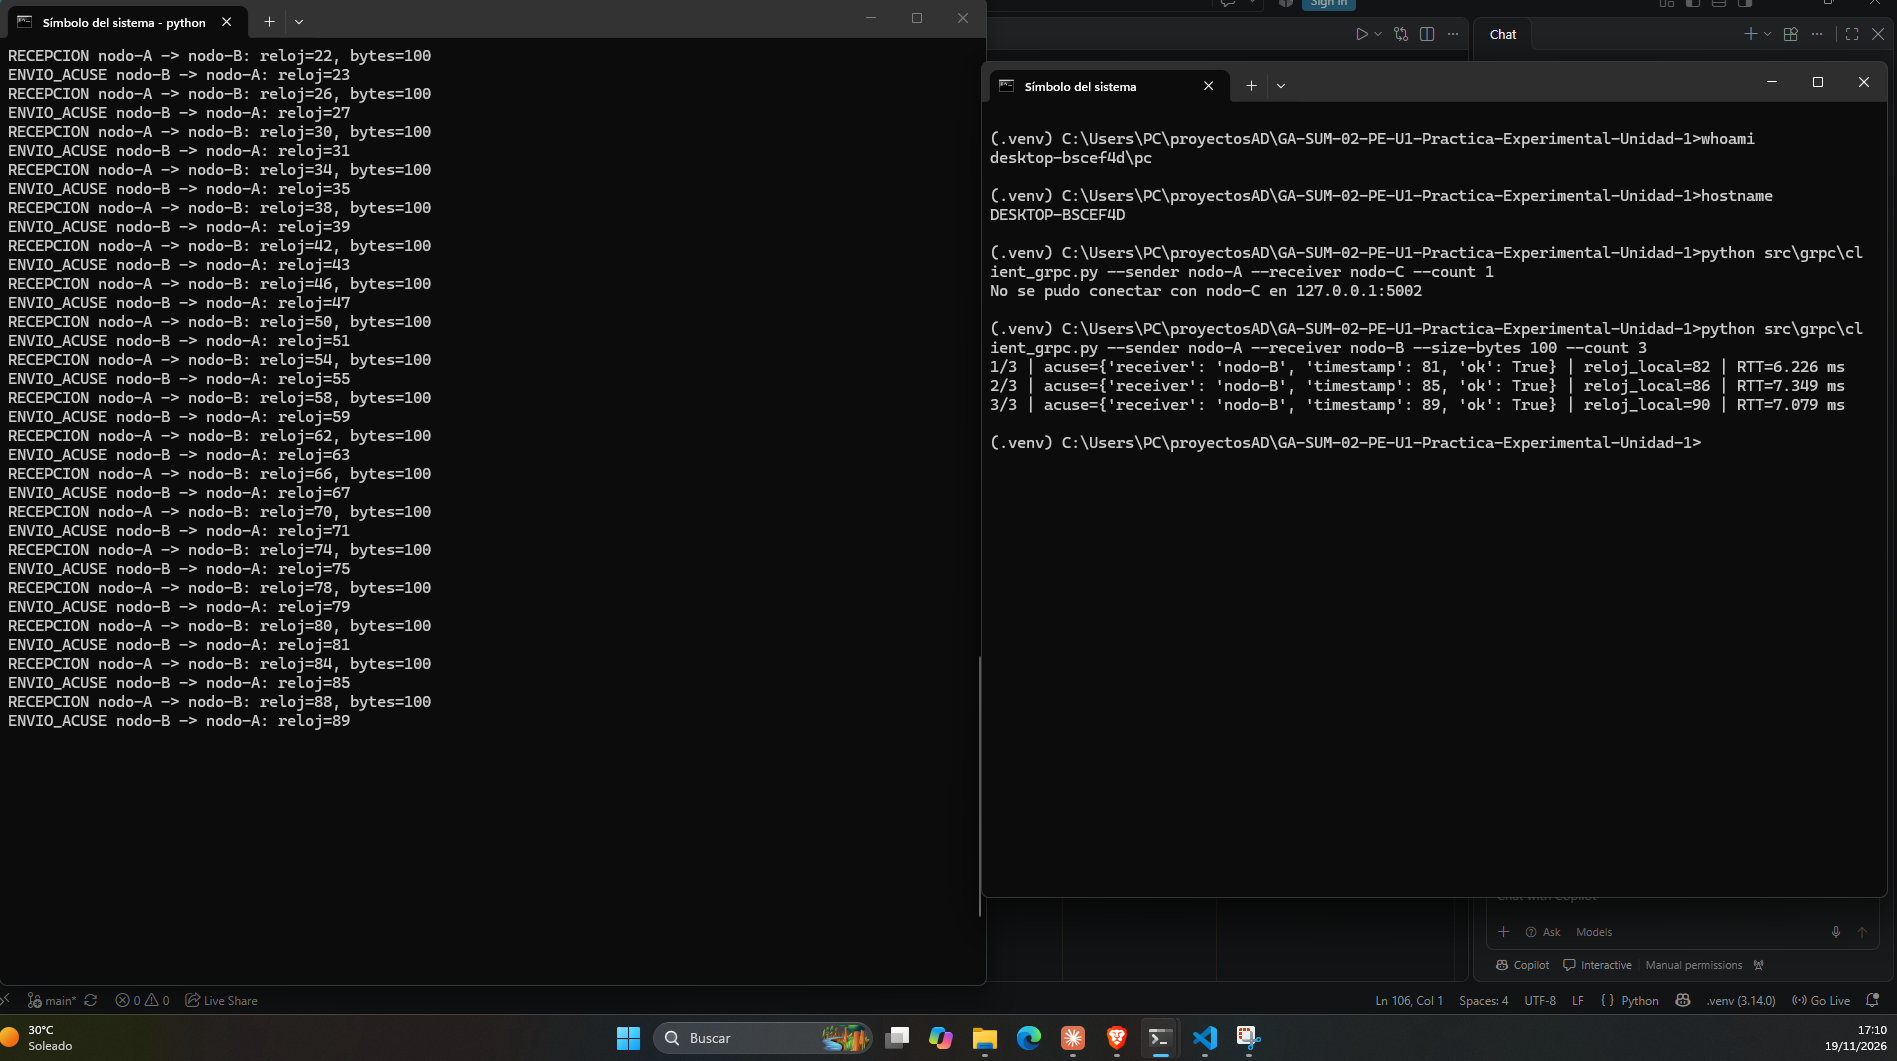
\includegraphics[width=\linewidth]{evidencias/Mera/grpc_nodo_caido_2026-11-19.png}
	\caption{Envío a \texttt{nodo-C} apagado y envíos correctos a \texttt{nodo-B} en la misma sesión.}
	\label{fig:grpc-nodo-caido}
\end{minipage}
\par\medskip

\subsubsection{Ejecución de 20 intercambios y registro de eventos}

Los 20 intercambios se ejecutaron el 19 de noviembre de 2026 con las mismas condiciones que la prueba TCP: servidor en \texttt{nodo-B}, cliente en \texttt{nodo-A}, carga de 100 bytes y corrida 0 (prueba funcional).

\begin{lstlisting}[language=bash,caption={Comandos de la prueba de 20 intercambios}]
	python src\grpc\server_grpc.py nodo-B
	python src\grpc\client_grpc.py --sender nodo-A --receiver nodo-B --size-bytes 100 --count 20 --run 0
\end{lstlisting}

Los 20 envíos recibieron acuse con \texttt{ok = True} (figura~\ref{fig:grpc-20}). En el primer intercambio, \texttt{nodo-A} envió con reloj 1, \texttt{nodo-B} registró la recepción con 2 y el envío del acuse con 3, y \texttt{nodo-A} quedó en 4 al recibirlo. Cada intercambio suma cuatro eventos, por lo que el último acuse llevó el valor 79 y el reloj de \texttt{nodo-A} terminó en 80. Es la misma secuencia que se obtuvo con TCP, lo que confirma que ambos mecanismos aplican las reglas de Lamport en el mismo orden; el transporte no cambia el resultado del reloj lógico. Las latencias de esta corrida (entre 6 y 32\,ms) no se usan en los resultados, porque el servidor imprimía y escribía en CSV en cada solicitud; las mediciones oficiales se obtuvieron con \texttt{analysis/benchmark.py} (sección de protocolo experimental).

\par\medskip
\noindent\begin{minipage}{\linewidth}
	\centering
	\makeatletter\def\@captype{figure}\makeatother
	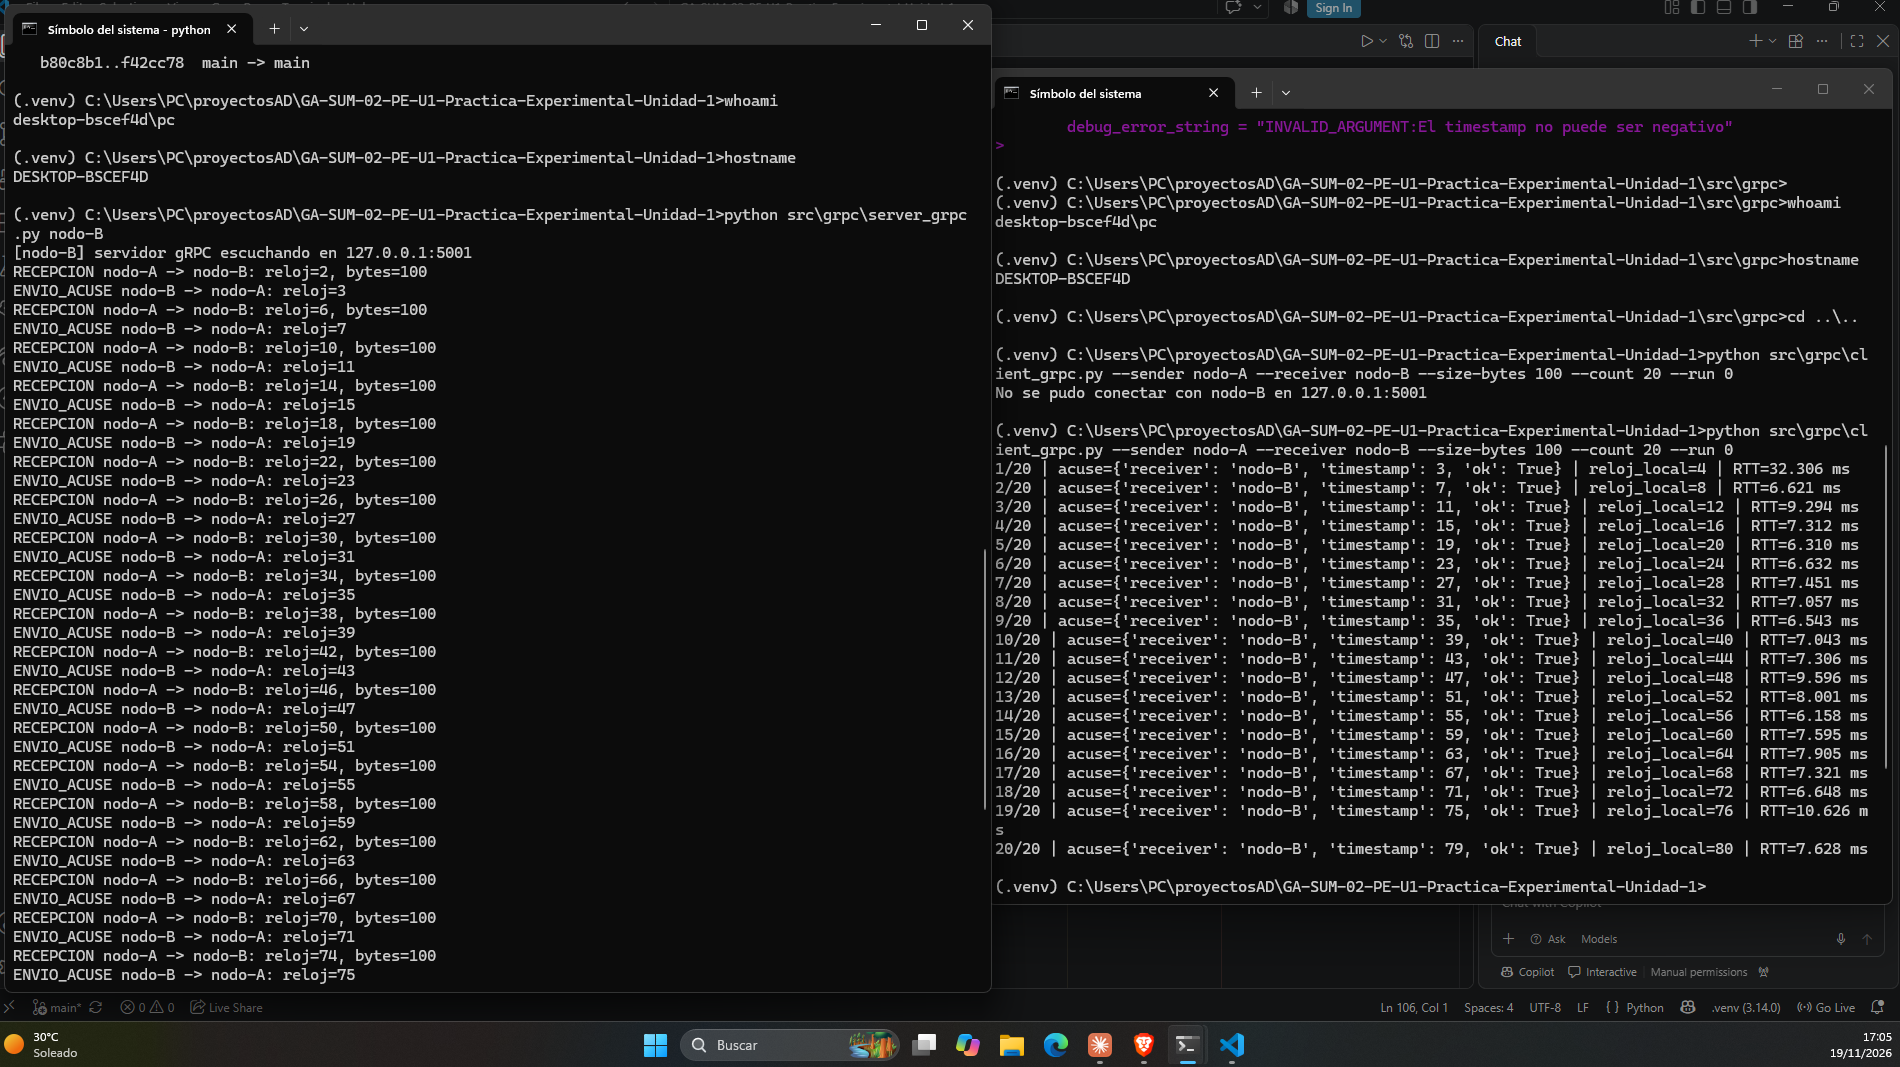
\includegraphics[width=\linewidth]{evidencias/Mera/grpc_20_intercambios_2026-11-19.png}
	\caption{Servidor gRPC de \texttt{nodo-B} (izquierda) y cliente de \texttt{nodo-A} (derecha) durante los 20 intercambios.}
	\label{fig:grpc-20}
\end{minipage}
\par\medskip

\pendiente{Indicar el archivo CSV de eventos gRPC de la corrida oficial que se usa en la verificación de Lamport, cuando el equipo lo genere y lo registre en SHA256SUMS. Los CSV de la corrida funcional del 19 de noviembre no se conservaron.}
% Desarrollo con asistencia de IA; pendiente de revisión del integrante responsable.
\subsection{Contador lógico por proceso}
El componente \path{src/common/lamport.py} define la clase
\texttt{LamportClock}. Cada nodo debe tener su propia instancia, compartida
entre los hilos de servidor y cliente del mismo proceso. No se comparte un
contador entre los tres nodos: eso eliminaría la independencia de sus relojes.
Dos procesos separados tampoco comparten esta instancia aunque utilicen el
mismo nombre de nodo.

Las operaciones de actualización y consulta usan un bloqueo de exclusión mutua.
El método \texttt{tick()} incrementa y devuelve el contador; \texttt{send()}
es una interfaz equivalente para envíos. La recepción valida primero que la
marca sea un entero no negativo y después aplica la regla de
la ecuación~\eqref{eq:lamport-recepcion}. Se rechazan valores booleanos aunque
Python los considere subtipos de entero. La propiedad \texttt{value} permite
consultar el reloj sin modificarlo.

El siguiente fragmento muestra la sección crítica de recepción:
\begin{lstlisting}[language=Python]
def receive(self, remote: int) -> int:
    _validate_timestamp(remote)
    with self._lock:
        self._value = max(self._value, remote) + 1
        return self._value
\end{lstlisting}

Para conservar compatibilidad de interfaces, el módulo también proporciona
\texttt{enviar()}, \texttt{recibir()} y \texttt{valor}. Los alias no representan
eventos adicionales: se elige una sola operación por evento. La compatibilidad
de nombres no demuestra por sí sola la integración con un transporte.

El cliente y el servidor TCP de esta revisión importan la clase común, en lugar
de mantener implementaciones locales duplicadas. Conservan sus argumentos de
ejecución y el formato JSON existente. El servidor y el cliente gRPC revisados
también importan la clase común y el servidor incrementa antes de enviar el acuse.
Esto unifica el algoritmo, pero los ejecutables actuales todavía crean instancias
separadas para cliente y servidor. No constituyen por sí solos una arquitectura
de tres procesos con servidor y cliente compartiendo reloj dentro de cada nodo.
El registro TCP existente también protege con un bloqueo la creación de cabecera
y la escritura de filas entre hilos del proceso. Este bloqueo evita escrituras
simultáneas, pero no garantiza que el orden de las filas coincida con el orden
de actualización de un reloj protegido por otro bloqueo independiente.

\subsection{Registro e identificación de eventos}
El componente propuesto en \path{src/common/event_log.py} implementa
\texttt{EventLog}. Su bloqueo engloba la actualización del reloj y la escritura
del evento, de modo que los hilos del proceso no registren una marca obtenida
por otra operación concurrente. El método devuelve exactamente la marca
registrada; ese retorno debe colocarse en el mensaje enviado.

\begin{lstlisting}[language=Python]
timestamp = log.record(
    "envio_solicitud", message_id, origin, destination)
# El transporte envia timestamp y message_id.
received = log.record(
    "recepcion_solicitud", message_id, origin,
    destination, remote=request_timestamp)
\end{lstlisting}

Como \texttt{record()} ya actualiza el contador, no se llama además a
\texttt{send()} o \texttt{receive()} para ese mismo evento. Durante una captura
completa, todos los eventos del reloj deben pasar por el registro y la captura
debe comenzar con el contador en cero.

El CSV contiene mecanismo, corrida, nodo, secuencia local, tipo de evento,
reloj local, reloj remoto cuando corresponde, hora UTC, identificador de
mensaje, origen y destino. La solicitud y su acuse comparten identificador,
pero sus tipos de evento permiten distinguir las dos direcciones. El ID debe
ser único por intercambio dentro de cada mecanismo y corrida y debe
transmitirse hasta el receptor; no se reconstruye a partir del orden de llegada.

Cada proceso escribe un archivo nuevo y exclusivo por corrida. La apertura
rechaza archivos existentes para evitar mezclar ejecuciones. La secuencia local
establece el orden del proceso; la hora UTC documenta cuándo se registró el
evento y no se utiliza como prueba de causalidad.

Este esquema corresponde al componente de registro preparado, no a los CSV
que producen actualmente los adaptadores del equipo. Sus registros existentes
no incluyen corrida, secuencia ni reloj remoto; el servidor gRPC reconstruye
los identificadores mediante contadores por emisor y conexión. Para emplear el
verificador completo se necesita integrar el registro y transmitir el ID real
desde el cliente. No es válido completar los CSV antiguos con valores supuestos.

\subsection{Concurrencia, validación y límites}
Las pruebas automatizadas comprueban actualizaciones sin pérdida entre hilos,
filas completas y secuencias ordenadas. El verificador
\path{analysis/verify_lamport.py} comprueba las reglas del contador y empareja
envíos y recepciones de solicitudes y acuses. También rechaza secuencias
incompletas, duplicados y marcas transmitidas inconsistentes.

El bloqueo no sincroniza procesos distintos ni protege automáticamente una
conexión de red compartida. Los adaptadores TCP y gRPC deben gestionar su
transporte y transmitir las marcas e identificadores del registro. Un fallo
de escritura invalida la captura y debe interrumpir esa corrida.

Un timeout no demuestra que el receptor no haya procesado la solicitud. Un
reintento no debe añadirse como si fuera el mismo intercambio completo: requiere
una política explícita de identificación y, si se pretende evitar efectos
duplicados, deduplicación en el receptor. El componente de reloj no implementa
esa política ni detecta fallos de nodos.

\pendiente{Integrar estos componentes en ambos transportes, ejecutar las pruebas
de tres clientes y fallos de nodos, y documentar los resultados reales. Las
pruebas unitarias no acreditan todavía esas ejecuciones.}


\section{Protocolo experimental}

% Autoría principal: Mario Zambrano.
% Protocolo de las mediciones realizadas el 20-11-2026.

\subsection{Entorno de ejecución}

El experimento se realizó el 20 de noviembre de 2026 en una computadora con Windows 11 Home
(versión 10.0.26200), procesador AMD Ryzen 7 7730U with Radeon Graphics y 15,34 GiB de
memoria RAM. Se utilizó Python 3.11.9 dentro de un entorno virtual para mantener las
dependencias del proyecto aisladas de otras instalaciones.

Las bibliotecas utilizadas fueron
\texttt{grpcio} y \texttt{grpcio-tools} 1.85.1,
\texttt{protobuf} 7.36.2, \texttt{pandas} 3.1.1
y \texttt{matplotlib} 3.11.2. Las versiones se
comprobaron antes de ejecutar las mediciones y
corresponden a las definidas en
\texttt{requirements.txt}.

La práctica contempla una arquitectura de tres
nodos independientes, denominados
\texttt{nodo-A}, \texttt{nodo-B} y
\texttt{nodo-C}, asociados a los puertos
5000, 5001 y 5002. Para la comparación de
rendimiento se utilizó el cliente identificado
como \texttt{nodo-A}, que estableció una
conexión con el servidor \texttt{nodo-B}
a través de \texttt{127.0.0.1:5001}.

Los mecanismos TCP y gRPC se evaluaron por separado, deteniendo el servidor anterior
antes de iniciar el siguiente. En ambos casos se redujo la salida por consola y
se desactivó el registro de eventos del servidor, mientras que los clientes
mantuvieron sus registros automáticos.

\subsection{Variables, condiciones y control experimental}

Se consideraron dos variables independientes: el mecanismo de comunicación y el tamaño de
la carga útil. Para el primer factor se evaluaron sockets TCP y gRPC con Protocol
Buffers; para el segundo se utilizaron mensajes de 100 y 10240 bytes.

Las cargas útiles se generaron mediante la repetición de un carácter ASCII. De esta
manera, el contenido enviado tuvo la longitud establecida para ambas
implementaciones. Los tamaños indicados corresponden únicamente al campo
\texttt{message} y no incluyen los bytes adicionales de JSON, Protocol Buffers ni
los encabezados de transporte.

La variable de respuesta principal fue la latencia de ida y vuelta (RTT), expresada
en milisegundos. Se midió el tiempo transcurrido durante la operación de
envío de una solicitud y recepción de su acuse, utilizando
\texttt{time.perf\_counter()}.

\begin{equation}
RTT_{\mathrm{ms}} =
(t_{\mathrm{fin}}-t_{\mathrm{inicio}})
\times 1000
\end{equation}

Como segunda métrica se calculó el rendimiento en mensajes por segundo. Para
cada corrida se dividió el número de mensajes confirmados entre la duración
total de dicha corrida:

\begin{equation}
R = \frac{N}{T}
\end{equation}

En esta expresión, $N$ representa la cantidad de mensajes confirmados y $T$
la duración de la corrida en segundos.

El benchmark reutilizó una conexión por mecanismo y tamaño de carga útil. Los
mensajes se enviaron secuencialmente: cada solicitud debía recibir su acuse
antes de continuar con la siguiente. Se estableció un tiempo de espera de
dos segundos por operación.

\subsection{Número de repeticiones y calentamiento}

La combinación de los dos mecanismos con los dos tamaños de mensaje produjo
cuatro condiciones experimentales.

Antes de cada condición se ejecutó una corrida de calentamiento de 100 envíos.
Estas observaciones quedaron excluidas de los archivos consolidados utilizados
para el análisis estadístico.

Después del calentamiento se realizaron cinco corridas medidas de 100 envíos,
equivalentes a 500 observaciones por condición.

\begin{table}[htbp]
\centering
\small
\begin{tabular}{lrrr}
\toprule
Mecanismo & Carga útil & Corridas & RTT medidos \\
\midrule
TCP  & 100 B   & 5 & 500 \\
TCP  & 10240 B & 5 & 500 \\
gRPC & 100 B   & 5 & 500 \\
gRPC & 10240 B & 5 & 500 \\
\midrule
\textbf{Total} & & \textbf{20} & \textbf{2000} \\
\bottomrule
\end{tabular}
\caption{Distribución de las mediciones del
experimento. Se excluyeron 400 envíos de
calentamiento.}
\label{tab:diseno_experimental}
\end{table}

Las corridas medidas finalizaron con 2000 acuses correctos. La revisión
posterior de los registros confirmó que cada condición contenía 500 RTT
positivos y válidos, distribuidos en cinco corridas de 100 mensajes.

\subsection{Prueba simultánea de tres clientes}

Además del benchmark secuencial, se realizaron pruebas funcionales utilizando tres nodos en localhost. Para ejecutarlas se utilizó \texttt{analysis/run\_lamport\_experiment.py}, que inicia tres procesos independientes. Cada proceso dispone de un servidor, un cliente y su propio reloj lógico de Lamport.

La comunicación se organizó en un anillo: el nodo-A envía solicitudes al nodo-B, el nodo-B al nodo-C y el nodo-C al nodo-A. Cada solicitud recibe un acuse de respuesta.

Como comprobación funcional se documentaron veinte intercambios por mecanismo, distribuidos entre los tres clientes en cantidades de 7, 7 y 6. Los registros correspondientes se conservaron en \texttt{data/lamport20/}, junto con los archivos de verificación y sus hashes SHA-256.

También se realizaron cuatro pruebas adicionales de concurrencia, combinando TCP y gRPC con cargas útiles de 100 y 10240 bytes. En cada condición se enviaron 300 solicitudes, distribuidas en partes iguales entre los tres clientes.

El lanzador utiliza barreras para coordinar el inicio de los servidores, el registro de los primeros envíos y la finalización. Este procedimiento permite estudiar eventos concurrentes, aunque no representa tráfico espontáneo ni demuestra que los envíos ocurrieran exactamente al mismo instante.

Las pruebas se ejecutaron en un entorno Linux diferente del equipo Windows utilizado para medir las latencias. Las cuatro capturas de 300 solicitudes fueron ejecuciones automatizadas asistidas, cuya procedencia y comandos se documentan en \texttt{data/concurrencia/PROCEDENCIA.md}. Las corridas personales de veinte intercambios se documentaron por separado mediante capturas.

Estos registros se utilizaron para verificar intercambios, acuses y relaciones causales mediante los relojes de Lamport. No se incorporaron a las 2000 mediciones RTT del benchmark, porque corresponden a condiciones y objetivos experimentales diferentes.


\subsection{Trazabilidad y protección de los datos}

Los resultados del benchmark se almacenaron en cuatro archivos CSV
dentro del directorio \texttt{data/}:

\begin{itemize}
    \item \texttt{latency\_sockets.csv}
    \item \texttt{runs\_sockets.csv}
    \item \texttt{latency\_grpc.csv}
    \item \texttt{runs\_grpc.csv}
\end{itemize}

Los archivos de latencia incluyen el mecanismo, tamaño del mensaje, corrida, intento, RTT, estado del acuse y fecha de registro. Los archivos de rendimiento contienen la duración de cada corrida, el número de mensajes confirmados y la tasa calculada en mensajes por segundo.

El análisis se realizó mediante \texttt{analysis/analisis\_resultados.py}, utilizando pandas y matplotlib. El programa comprobó la estructura de los datos, la cantidad de registros por condición y la ausencia de acuses fallidos o latencias inválidas. A partir de los archivos originales generó los resúmenes estadísticos, las tablas LaTeX y las figuras.

Los CSV consolidados se conservaron sin modificaciones manuales. También se calcularon sus huellas SHA-256, registradas en \texttt{data/SHA256SUMS}. La integridad se comprobó recalculando cada hash y comparándolo con su valor almacenado.

Los archivos automáticos \texttt{latencias\_*.csv} y \texttt{eventos\_*.csv} se mantuvieron separados de las mediciones consolidadas, ya que contienen también registros de calentamiento y pruebas funcionales.

\subsection{Limitaciones y amenazas a la validez}

Las mediciones se realizaron en localhost, por lo que no incorporan las condiciones de una comunicación entre computadoras a través de una red física. Factores como la latencia de red, la congestión o la variabilidad de los enlaces podrían modificar los resultados en otro entorno.

Aunque ambos mecanismos utilizaron las mismas cargas útiles, sus operaciones internas no fueron idénticas. En TCP, la serialización JSON se realizó dentro del intervalo medido. En gRPC, el objeto de solicitud se construyó antes de iniciar el cronómetro y la llamada remota quedó incluida en la medición. En consecuencia, las diferencias observadas corresponden a las implementaciones evaluadas y no pueden atribuirse exclusivamente al protocolo de transporte.

También deben distinguirse las métricas utilizadas. El RTT individual no incluye todas las operaciones de registro posteriores a la recepción del acuse, mientras que el rendimiento considera la duración completa de cada corrida, incluyendo dichas operaciones.

Las pruebas TCP se ejecutaron antes que las de gRPC. No se controló instrumentalmente la actividad de otros procesos de Windows ni la variación de carga del procesador. La planificación de tareas del sistema operativo y otras actividades en segundo plano pudieron influir en los tiempos obtenidos.

Por estas razones, los resultados permiten comparar el comportamiento de los clientes implementados por el equipo bajo las condiciones específicas de esta práctica, sin establecer conclusiones generales sobre el rendimiento de TCP y gRPC en cualquier sistema distribuido.

\section{Resultados de las mediciones}

% Autoría principal: Mario Zambrano.

\subsection{Estadísticas descriptivas por mecanismo y tamaño}

Se analizaron 2000 mediciones de latencia RTT, distribuidas
entre TCP y gRPC con mensajes de 100 y 10240 bytes.
Para cada combinación se realizaron cinco corridas
de 100 envíos, obteniendo 500 mediciones por caso.

A partir de los archivos CSV se calcularon la media,
mediana, desviación estándar y percentil 95 (P95).
Estos cálculos se realizaron mediante el script
\texttt{analisis\_resultados.py}, utilizando pandas.
Los resultados se muestran en la
Tabla~\ref{tab:estadisticas_rtt}.

\begin{table}[htbp]
\centering
\small
\resizebox{\linewidth}{!}{%
\begin{tabular}{llrrrrr}
\toprule
Mecanismo & Carga útil & $n$ & Media (ms) & Mediana (ms) & DE (ms) & P95 (ms) \\
\midrule
TCP & 100 B & 500 & 0.122 & 0.113 & 0.028 & 0.185 \\
TCP & 10 KiB (10240 B) & 500 & 0.197 & 0.186 & 0.039 & 0.282 \\
gRPC & 100 B & 500 & 0.547 & 0.489 & 0.231 & 0.819 \\
gRPC & 10 KiB (10240 B) & 500 & 0.564 & 0.533 & 0.110 & 0.758 \\
\bottomrule
\end{tabular}%
}
\caption{Latencia RTT por mecanismo y tamaño de carga útil. DE: desviación estándar muestral; P95: percentil 95.}
\label{tab:estadisticas_rtt}
\end{table}


En las pruebas realizadas, TCP presentó una latencia
media menor que gRPC con los dos tamaños de mensaje.
Lo mismo ocurrió con las medianas y los valores del
percentil 95.

Al aumentar el tamaño del mensaje de 100 a 10240 bytes,
la latencia media también aumentó en ambos casos.
Este cambio fue mayor en TCP, mientras que en gRPC
la diferencia entre los dos tamaños fue más pequeña.

También se encontraron diferencias en la dispersión
de los tiempos. gRPC registró una desviación estándar
mayor que TCP, especialmente con mensajes de 100 bytes.
Esto indica que sus tiempos de respuesta fueron menos
uniformes durante las pruebas.

Las posibles razones de estas diferencias se
analizarán en la sección de discusión.

\subsection{Rendimiento: mensajes por segundo}

Además de medir la latencia, se calculó cuántos mensajes
podía procesar cada implementación por segundo.
Para ello, se dividió la cantidad de mensajes
confirmados entre el tiempo total de cada corrida.

En la Tabla~\ref{tab:rendimiento} se presentan
los promedios de rendimiento y sus desviaciones
estándar, calculados a partir de las cinco
corridas realizadas para cada caso.

\begin{table}[htbp]
\centering
\small
\resizebox{\linewidth}{!}{%
\begin{tabular}{llrrr}
\toprule
Mecanismo & Carga útil & Corridas & Media (mensajes/s) & DE (mensajes/s) \\
\midrule
TCP & 100 B & 5 & 576.43 & 4.03 \\
TCP & 10 KiB (10240 B) & 5 & 533.24 & 17.70 \\
gRPC & 100 B & 5 & 442.64 & 21.42 \\
gRPC & 10 KiB (10240 B) & 5 & 431.98 & 19.71 \\
\bottomrule
\end{tabular}%
}
\caption{Rendimiento observado, calculado como mensajes confirmados divididos entre la duración de cada corrida; media y desviación estándar de cinco corridas.}
\label{tab:rendimiento}
\end{table}


TCP obtuvo un rendimiento medio superior al de gRPC
con ambos tamaños de mensaje. También se observó
que el número de mensajes procesados por segundo
disminuyó al utilizar la carga de 10240 bytes.

En cuanto a la variación entre corridas, TCP con
mensajes de 100 bytes presentó los resultados más
uniformes. Por su parte, gRPC registró diferencias
mayores entre las repeticiones.

Es importante aclarar que el rendimiento y el RTT
no se calculan de la misma manera. El rendimiento
considera el tiempo completo de cada corrida,
incluyendo las operaciones de registro realizadas
por el cliente. Por eso, no se obtiene simplemente
dividiendo uno entre la latencia media.

\subsection{Gráfico de cajas de latencias}

Para observar mejor la distribución de los tiempos,
se generó el diagrama de cajas de la
Figura~\ref{fig:boxplot}. Este gráfico permite
comparar las medianas, la dispersión y los
valores atípicos de las mediciones.

\begin{figure}[H]
    \centering
    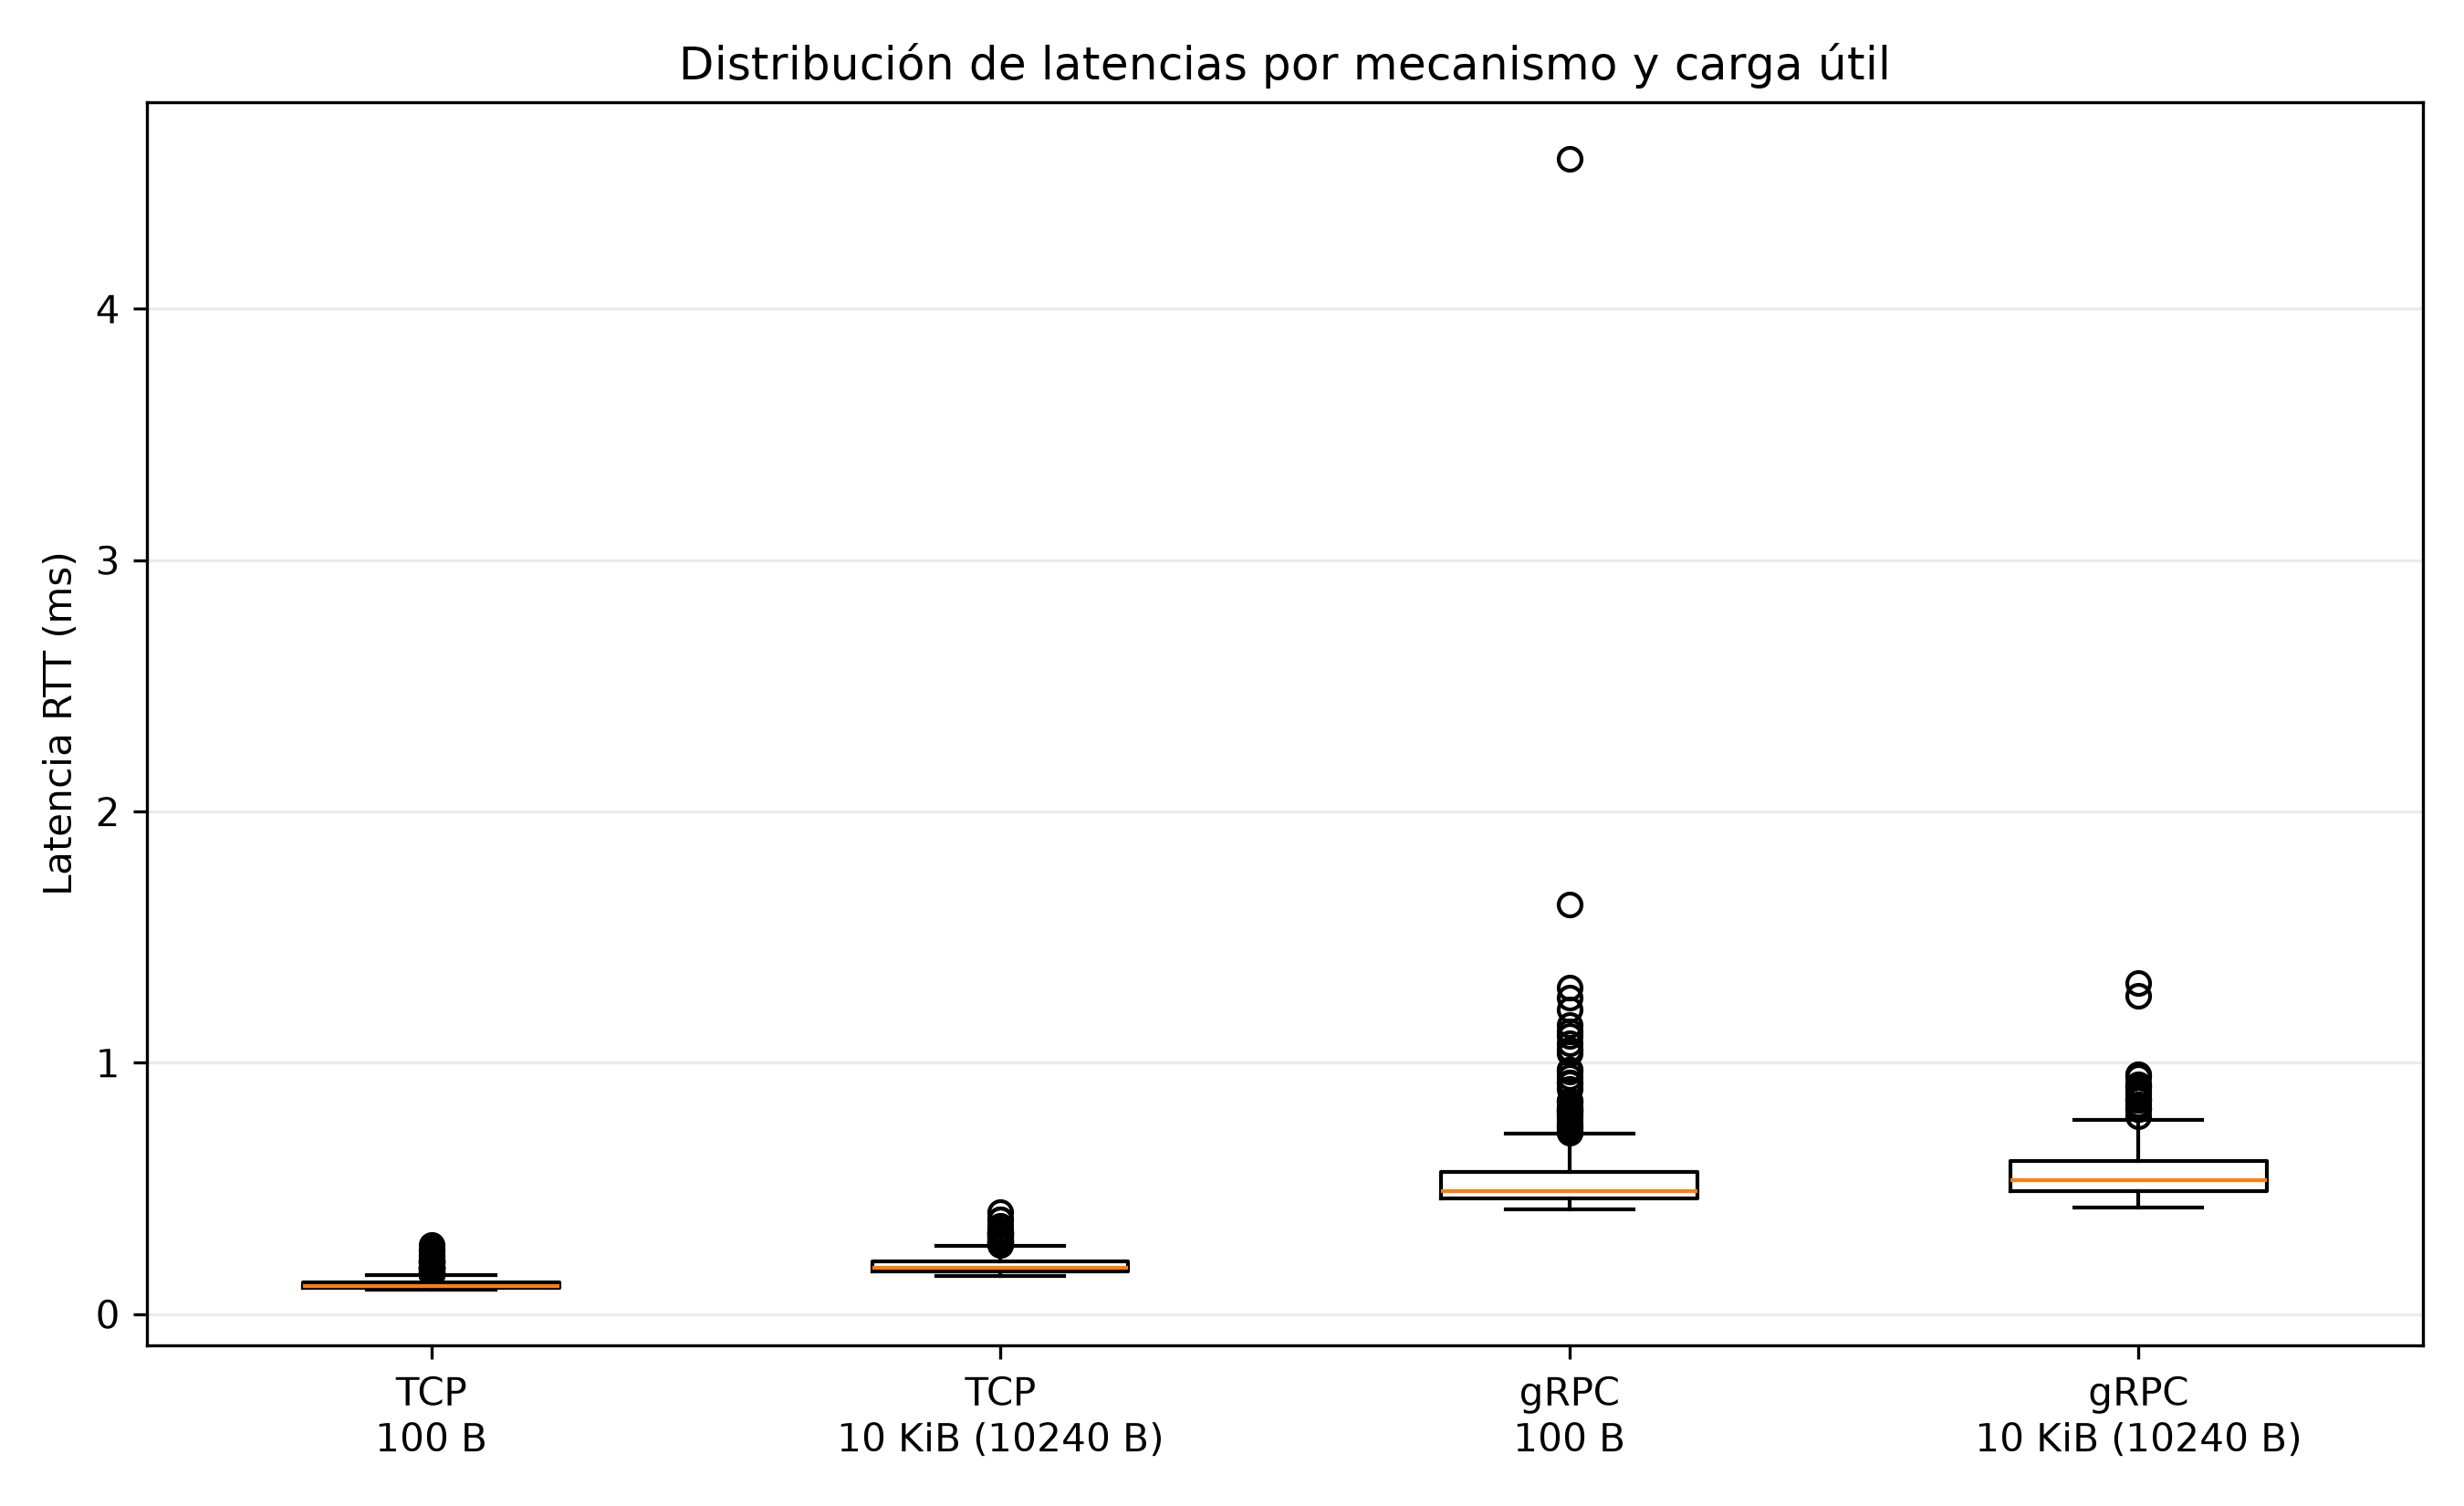
\includegraphics[width=0.95\linewidth]
    {figures/boxplot.png}
    \caption{Distribución de las latencias RTT de
    TCP y gRPC con mensajes de 100 bytes y 10 KiB.
    Gráfico generado a partir de los CSV originales.}
    \label{fig:boxplot}
\end{figure}

Como se observa en el gráfico, los tiempos de TCP
se concentran en valores más bajos que los de gRPC.
También se aprecia que las mediciones de gRPC
presentan una mayor dispersión, principalmente
con mensajes de 100 bytes.

En esta última condición aparecen algunos valores
atípicos que se alejan del resto de las mediciones.
Se decidió conservarlos porque forman parte de
los datos obtenidos durante la ejecución.
Por tanto, también se consideraron en los
cálculos estadísticos.

El gráfico permite identificar estas diferencias,
pero no es suficiente para determinar qué provocó
cada aumento de latencia.

\subsection{Gráfico de barras con intervalos}

La Figura~\ref{fig:barras} muestra una comparación
de la latencia media para los dos mecanismos y
los dos tamaños de mensaje.

Cada barra representa el promedio de las cinco
medias obtenidas por corrida. Las líneas verticales
indican una desviación estándar por encima y por
debajo de ese promedio, calculada entre las
cinco corridas.

\begin{figure}[H]
    \centering
    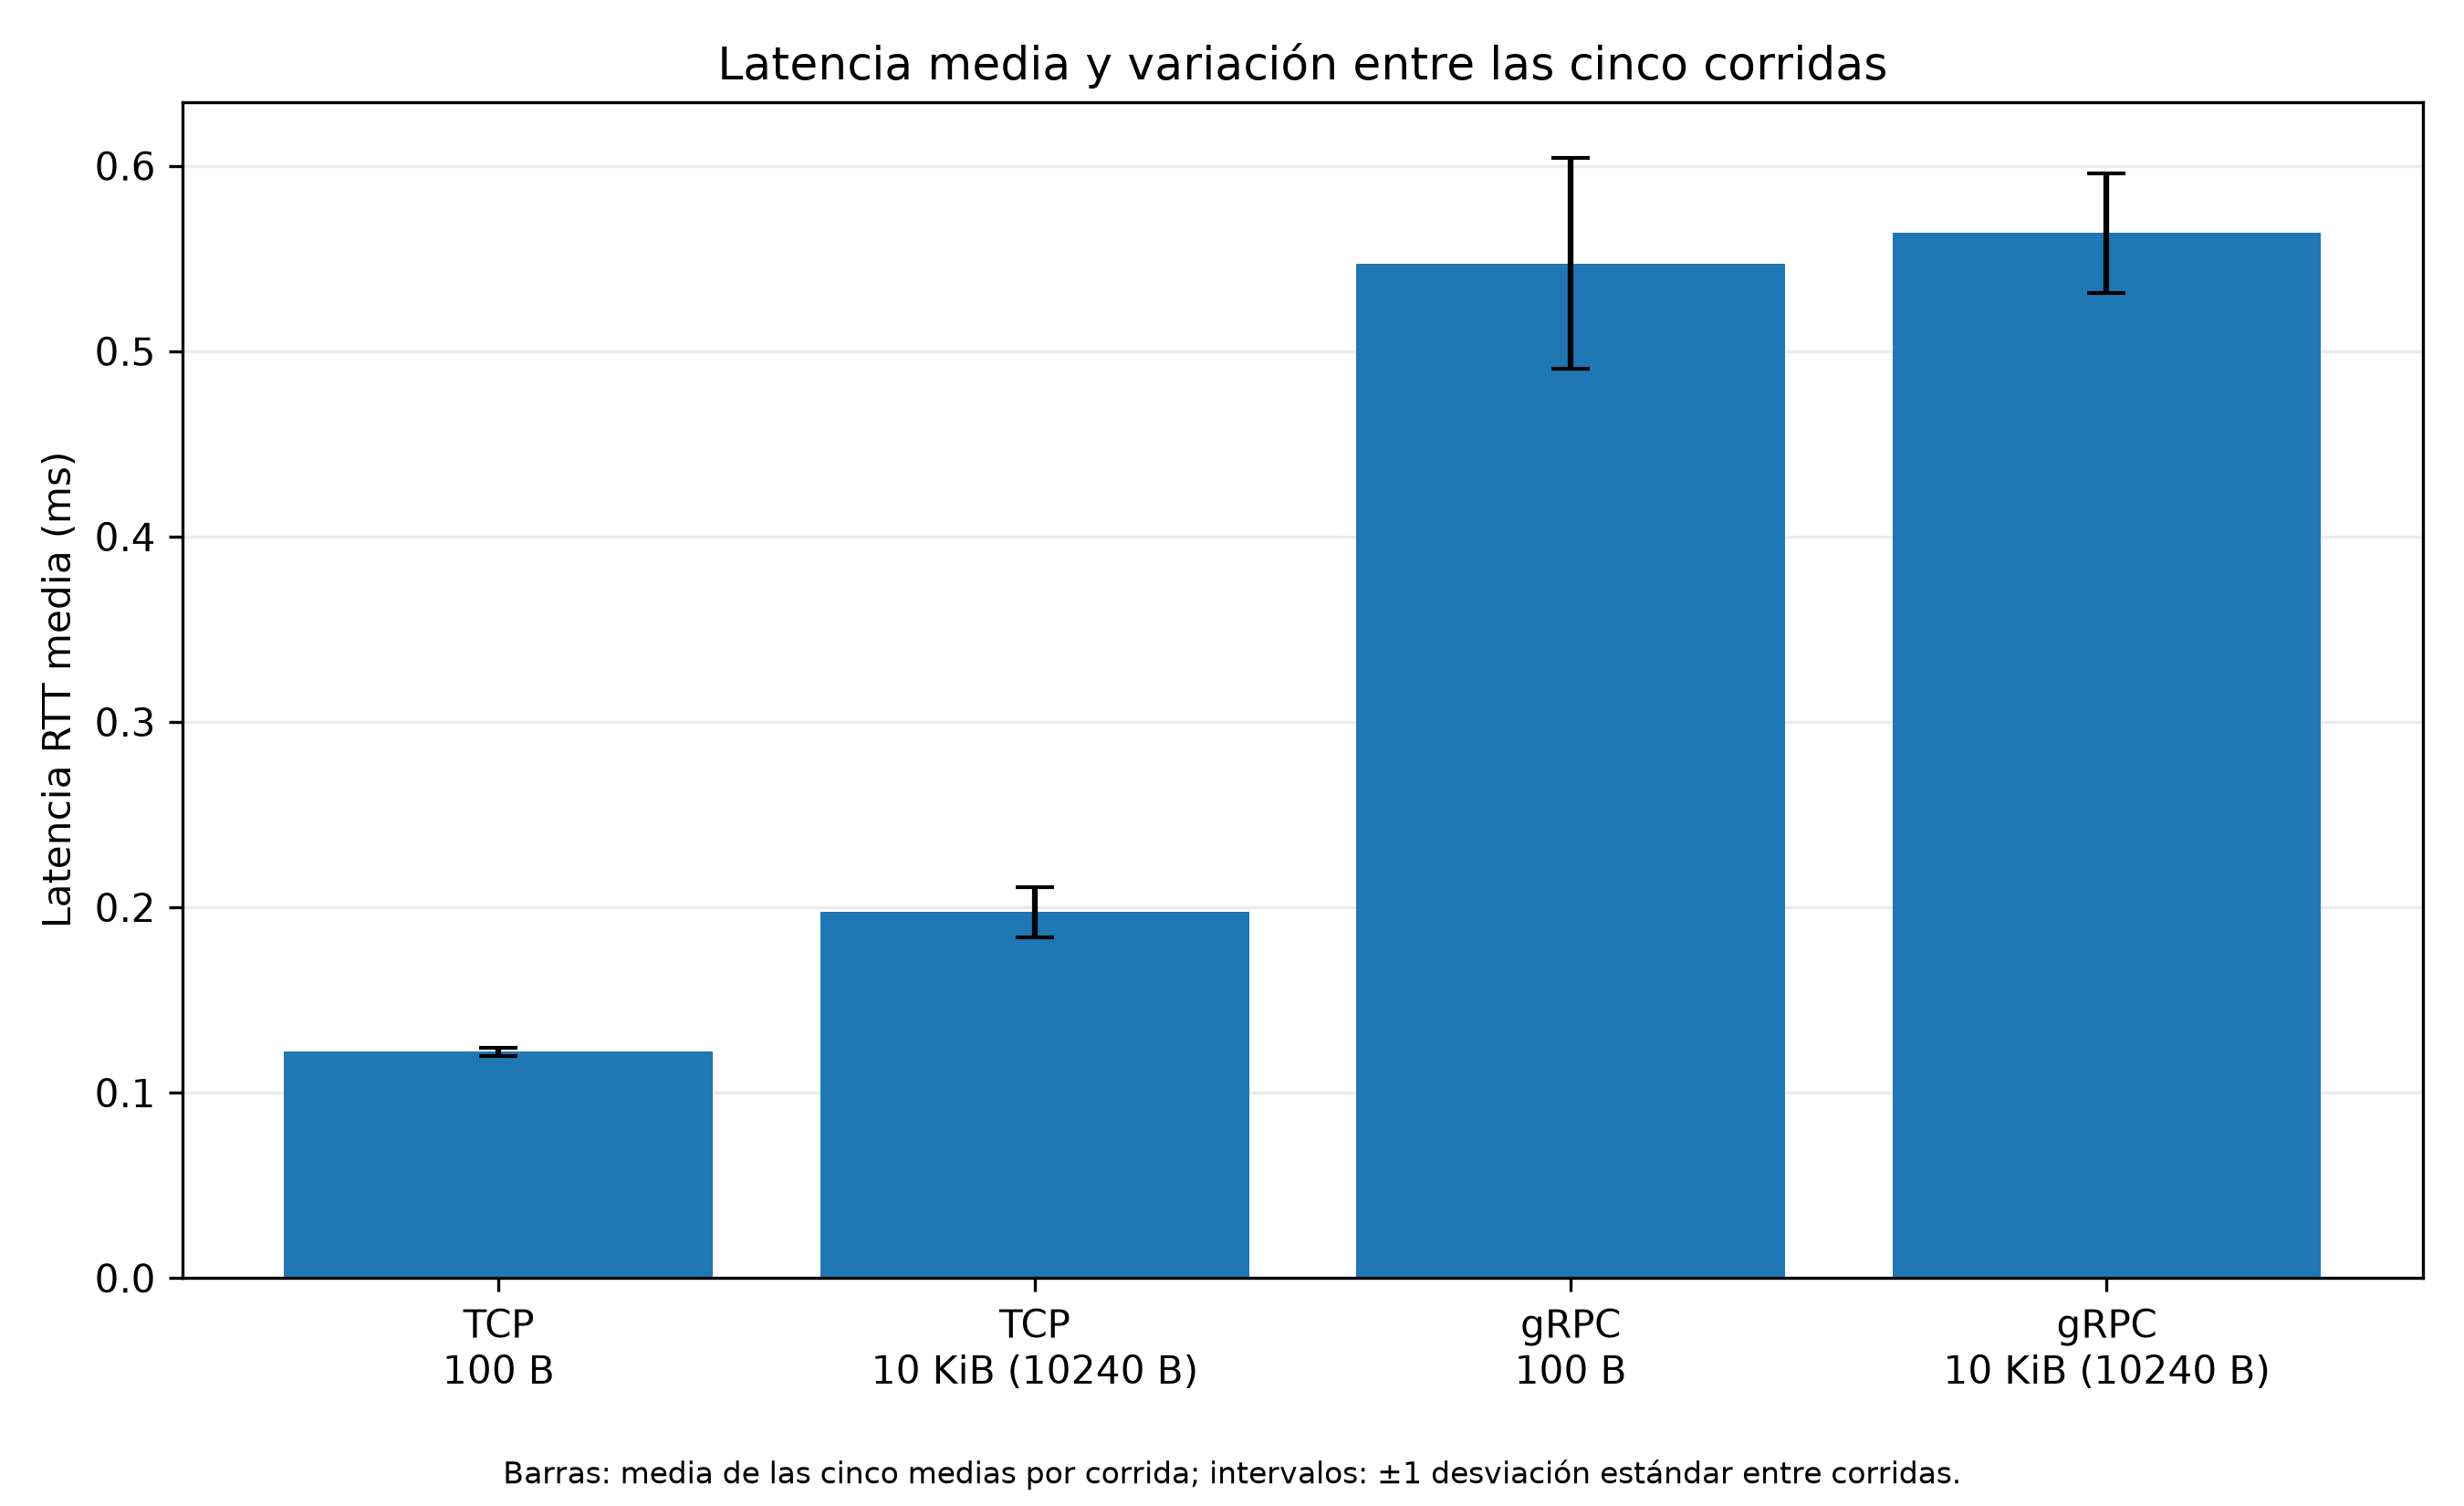
\includegraphics[width=0.85\linewidth]
    {figures/barras_intervalos.png}
    \caption{Comparación de las latencias medias.
    Los intervalos representan $\pm 1$ desviación
    estándar entre las cinco corridas y no son
    intervalos de confianza del 95\%.}
    \label{fig:barras}
\end{figure}

En el gráfico se puede observar que TCP mantuvo
una latencia media inferior a gRPC con los dos
tamaños de mensaje.

Las líneas de dispersión muestran que los tiempos
no fueron exactamente iguales en todas las
corridas. Esto se aprecia especialmente en gRPC
con mensajes de 100 bytes, donde hubo una mayor
diferencia entre las medias de las repeticiones.

Estos intervalos sirven para mostrar cuánto
variaron los resultados entre corridas.
No se utilizaron para realizar una prueba
de significación estadística.

\subsection{Alcance de los resultados y concurrencia}

Las veinte corridas del benchmark se completaron
correctamente. En los archivos consolidados
se registraron 2000 mediciones válidas,
sin acuses fallidos ni latencias inválidas.

Estos valores corresponden a mensajes enviados
de forma secuencial entre el cliente
\texttt{nodo-A} y el servidor \texttt{nodo-B}.
Por tanto, las cifras de latencia y rendimiento
presentadas anteriormente no describen por
sí solas el comportamiento con tres clientes
concurrentes.

En las pruebas funcionales posteriores se
registraron veinte intercambios por mecanismo,
con tres nodos en funcionamiento. Tanto TCP
como gRPC completaron las veinte solicitudes
y sus acuses. Cada ejecución produjo 80
eventos y 40 pares de envío y recepción,
sin errores causales en el informe de
verificación.

Para evaluar la concurrencia se realizaron
cuatro pruebas adicionales, con cargas de
100 y 10240 bytes para ambos mecanismos.
En cada condición se registraron 300
solicitudes, 300 acuses y 1200 eventos.
Los informes de verificación no reportaron
errores causales en estas capturas.

Estos resultados muestran que las
implementaciones completaron los intercambios
registrados bajo las condiciones probadas.
Aunque las pruebas con tres clientes se completaron
correctamente, no se utilizaron para comparar
latencias ni mensajes por segundo con el benchmark
inicial. Su objetivo fue comprobar la comunicación
entre los nodos y verificar los relojes de Lamport,
además de haberse ejecutado en un entorno diferente.

La verificación de las reglas de Lamport,
los ejemplos de eventos concurrentes y
la procedencia de los registros se
presentan con mayor detalle en la
sección de verificación del reloj lógico.



\section{Discusión y análisis crítico}

% Autoría compartida: Mario coordina la discusión.

\subsection{Comparación de latencia, dispersión y rendimiento}

Los resultados obtenidos permiten identificar diferencias
entre ambas implementaciones bajo las condiciones del
experimento. En las mediciones secuenciales sobre localhost,
TCP presentó menores tiempos de respuesta que gRPC con los
dos tamaños de mensaje evaluados.

Con cargas de 100 bytes, la latencia media fue de
0,122\,ms para TCP y 0,547\,ms para gRPC. Esto significa
que el promedio de gRPC fue aproximadamente 4,48 veces
el de TCP. Al utilizar mensajes de 10\,KiB, las medias
aumentaron a 0,197\,ms y 0,564\,ms, respectivamente,
reduciéndose la relación a aproximadamente 2,86 veces.
Estos valores se presentan en la
Tabla~\ref{tab:estadisticas_rtt}.

También se observó un comportamiento diferente al
incrementar el tamaño de la carga útil. La latencia
media de TCP aumentó alrededor de un 61,5\,\%,
mientras que en gRPC el incremento fue cercano
al 3,1\,\%. Aunque esto muestra una menor variación
de la media de gRPC entre los tamaños probados,
no demuestra que tenga mejor escalabilidad en
cualquier situación. Para establecerlo sería
necesario evaluar más tamaños y condiciones de carga.

La dispersión aporta otra perspectiva. Con mensajes
de 100 bytes, gRPC registró una desviación estándar
de 0,231\,ms, frente a 0,028\,ms en TCP. Además,
el percentil 95 fue de 0,819\,ms para gRPC y
0,185\,ms para TCP. Esto indica que la diferencia
no se limitó a los promedios: también hubo una
mayor variación en los tiempos de gRPC durante
esa condición.

Con mensajes de 10\,KiB, las desviaciones estándar
fueron de 0,039\,ms para TCP y 0,110\,ms para gRPC.
Los percentiles 95 se situaron en 0,282\,ms y
0,758\,ms, respectivamente. Por tanto, TCP mantuvo
tiempos más bajos en las medidas de tendencia
central y en el extremo superior de la
distribución observado mediante el P95.

En cuanto al rendimiento, TCP alcanzó una media
de 576,43 mensajes por segundo con 100 bytes,
frente a 442,64 en gRPC. Para 10\,KiB se
registraron 533,24 y 431,98 mensajes por segundo,
respectivamente. En las condiciones evaluadas,
el rendimiento de TCP fue aproximadamente un
30,2\,\% superior con 100 bytes y un 23,4\,\%
superior con 10\,KiB
(Tabla~\ref{tab:rendimiento}).

Estas diferencias deben interpretarse considerando
cómo se implementaron las mediciones. TCP construye
y serializa directamente sus mensajes JSON, mientras
que gRPC utiliza clases generadas a partir de
Protocol Buffers y realiza llamadas remotas sobre
HTTP/2. Por ello, la comparación refleja el
comportamiento conjunto de las implementaciones,
sus bibliotecas y sus operaciones auxiliares,
no únicamente el costo del protocolo de transporte.

Las pruebas posteriores con tres nodos complementan
estos resultados desde el punto de vista funcional.
En las corridas de veinte intercambios, tanto TCP
como gRPC completaron las solicitudes y sus acuses.
Asimismo, las cuatro capturas concurrentes de
300 solicitudes registraron 1200 eventos por
condición, sin errores causales reportados por
el verificador de Lamport.

Sin embargo, estas pruebas utilizaron otro entorno
y tuvieron como propósito comprobar la comunicación
y el orden causal de los eventos. Por ello, no se
emplearon para ampliar las muestras de latencia
ni para comparar mensajes por segundo con el
benchmark secuencial.

\subsection{Facilidad de desarrollo, tipado y manejo de errores}

% Parte gRPC (Mera).
En gRPC, antes de programar hubo que definir el contrato \texttt{messaging.proto} y generar el código con \texttt{grpcio-tools}, que debe regenerarse ante cualquier cambio. A cambio, el servidor solo implementa \texttt{EnviarMensaje} y el cliente lo invoca desde el stub, sin construir ni leer los mensajes, como sí ocurre en TCP con el JSON y el salto de línea. La principal dificultad fue de organización: para usar el reloj compartido de \texttt{src/common/} hubo que agregar la raíz del repositorio a \texttt{sys.path}.

El contrato garantiza los tipos, por lo que el servidor gRPC no necesita las comprobaciones con \texttt{isinstance} del servidor TCP. Sin embargo, no reemplaza toda la validación: un \texttt{timestamp} negativo llega como entero válido y lo rechaza el reloj, y en proto3 un campo omitido toma su valor por defecto \cite{protobufProto3}, de modo que una solicitud sin \texttt{timestamp} llegó con valor 0 sin ningún error. En los fallos, gRPC devuelve códigos estándar con descripción: el cliente recibió \texttt{INVALID\_ARGUMENT} y el servidor siguió atendiendo, mientras que en TCP una solicitud mal formada cierra la conexión sin informar la causa. Como contrapartida, los mensajes binarios no se pueden leer a simple vista al depurar.

Esta comodidad tiene un costo (tabla~\ref{tab:estadisticas_rtt}): con 100 bytes, la latencia media de gRPC fue unas 4,5 veces la de TCP (0,547\,ms frente a 0,122\,ms). Con 10\,KiB, TCP subió un 61\,\% y gRPC solo un 3\,\%, lo que sugiere que el costo adicional de gRPC es principalmente fijo por llamada.

Desde TCP, la comunicación fue directa de implementar: el cliente abre una conexión con el servidor y la reutiliza para enviar varios mensajes. Sin embargo, como TCP transmite un flujo de bytes, tuvimos que definir en el código cómo separar cada solicitud. Para eso usamos objetos JSON codificados en UTF-8 y un salto de línea al final de cada mensaje. El cliente también construye y analiza manualmente el JSON, mientras que el servidor valida los campos recibidos. Esto nos dio control sobre el intercambio, pero exigió mantener el mismo formato y las mismas reglas en ambos extremos.

El tipado queda a cargo de esas validaciones: por ejemplo, se comprueba que el emisor y el mensaje sean textos, que la marca de tiempo sea un entero y que el acuse tenga los campos esperados. En el manejo de errores, el cliente distingue situaciones como un tiempo de espera agotado, una conexión rechazada u otro error de comunicación. Si la solicitud recibida no tiene el formato esperado, el servidor no devuelve un error estructurado para la aplicación y puede cerrar esa conexión. En esta implementación, TCP requirió más trabajo manual para definir el formato, validar los datos y tratar los errores que la interfaz gRPC generada a partir de su contrato.

\subsection{Contraste con la hipótesis inicial}

La hipótesis planteada antes de realizar las mediciones
establecía que la implementación con sockets TCP
presentaría una latencia media menor que gRPC en
localhost, tanto para mensajes de 100 bytes como
para mensajes de 10240 bytes.

Los resultados respaldaron esta expectativa dentro
de las condiciones estudiadas. Con cargas de 100 bytes,
TCP obtuvo una media de 0,122\,ms, inferior a los
0,547\,ms de gRPC. La misma relación se mantuvo
con 10\,KiB, donde TCP registró 0,197\,ms y
gRPC 0,564\,ms.

Estos resultados cumplen el criterio que se había
establecido previamente para considerar respaldada
la hipótesis. Además, las medianas y los percentiles
95 mantuvieron la misma tendencia, por lo que la
diferencia observada no dependió únicamente de
los valores medios.

No obstante, la hipótesis debe aceptarse solo
dentro de su alcance experimental. Las mediciones
se realizaron en una computadora, con comunicación
local y mediante implementaciones específicas
desarrolladas por el equipo. Tampoco se aplicó
una prueba de significación estadística para
generalizar las diferencias a otras poblaciones
de ejecuciones.

En consecuencia, los resultados respaldan la
hipótesis inicial para nuestro experimento,
pero no permiten afirmar que los sockets TCP
ofrezcan siempre menor latencia que gRPC
en cualquier aplicación distribuida.

\subsection{Aplicación posible al Proyecto Fin de Curso}

El Proyecto Fin de Curso de un integrante del equipo corresponde
al Sistema de Gestión de Refuerzo Académico
(SGRA), una aplicación web orientada a gestionar
solicitudes de refuerzo, disponibilidad docente,
sesiones académicas, notificaciones y seguimiento
de los estudiantes.

Su arquitectura contempla una interfaz desarrollada
con Angular, un backend con Spring Boot y una
base de datos PostgreSQL. La comunicación entre
el frontend y el backend se realiza mediante
una API REST sobre HTTP. Por tanto, la práctica
no implica sustituir automáticamente esta
arquitectura por TCP o gRPC.

Si el SGRA evolucionara hacia servicios de
backend independientes, gRPC podría evaluarse
para la comunicación interna entre componentes.
Por ejemplo, un servicio encargado de gestionar
solicitudes de refuerzo podría consultar a
otro servicio los datos académicos necesarios
para validar asignaturas, docentes o
disponibilidad.

En ese escenario, Protocol Buffers permitiría
establecer contratos explícitos para las
solicitudes y respuestas. Además, los códigos
de estado y los límites de tiempo de gRPC
ofrecerían mecanismos definidos para gestionar
errores de comunicación. Esta sería una
alternativa de diseño que requeriría pruebas
propias antes de adoptarse.

Por otro lado, los sockets TCP podrían utilizarse
en un componente interno muy específico que
necesitara intercambiar mensajes simples mediante
un protocolo controlado por el equipo, como un
mecanismo experimental de supervisión de
conectividad. Sin embargo, habría que implementar
la delimitación, validación, autenticación y
gestión de errores de esos mensajes.

Por estas razones, no sería conveniente reemplazar
la API REST del SGRA por sockets TCP personalizados
solo porque estos presentaron menor latencia en
nuestra práctica. Para operaciones como registrar
solicitudes, consultar historiales o gestionar
usuarios, también deben considerarse la seguridad,
el mantenimiento y la integración con el frontend.

En cuanto al teorema CAP, su aplicación depende
de las garantías de consistencia y disponibilidad
de los datos distribuidos, no de escoger TCP
o gRPC. Si en el futuro el SGRA incorporara
réplicas de información académica o de solicitudes,
sería necesario definir cómo actuar ante
interrupciones de comunicación entre ellas.

Por ejemplo, una solicitud de refuerzo no debería
quedar confirmada dos veces por utilizar copias
inconsistentes de los mismos datos. Este problema
requiere decisiones sobre almacenamiento,
transacciones y coordinación, independientemente
del mecanismo empleado para transportar mensajes.

En definitiva, los resultados experimentales
sirven como referencia para analizar alternativas
de comunicación, pero la elección tecnológica
para el SGRA debe partir de sus requisitos
funcionales, de seguridad y de despliegue.

\subsection{Amenazas a la validez y propuestas de mejora}

La principal limitación del benchmark es que las
mediciones se realizaron sobre localhost. Esto
eliminó factores propios de una red entre equipos,
como la congestión, los retardos de transmisión
entre dispositivos y las pérdidas de conectividad.
Por tanto, las latencias obtenidas no representan
necesariamente las que se observarían en un
despliegue real.

Otro aspecto importante es que las condiciones
de medición no incluyeron exactamente las mismas
operaciones internas. En TCP, la serialización
JSON quedó dentro del intervalo medido, mientras
que en gRPC el objeto de solicitud se construyó
antes de iniciar el cronómetro. Además, cada
implementación utiliza bibliotecas y formatos
de mensajes diferentes. Esto limita la posibilidad
de atribuir las diferencias a una sola causa.

El orden de ejecución también pudo influir,
ya que las pruebas TCP se realizaron antes
que las de gRPC. No se midió de manera
instrumental la actividad de otros procesos
ni se controlaron todas las variaciones
de carga del sistema operativo.

Aunque se obtuvieron 500 mediciones por
condición, estas proceden de cinco corridas
consecutivas de cien solicitudes. Los valores
tomados dentro de una misma corrida pueden
compartir condiciones temporales, por lo que
no deben interpretarse automáticamente como
500 repeticiones completamente independientes.

También se utilizaron únicamente dos tamaños
de carga útil, generados mediante caracteres
ASCII repetidos. Esta decisión permitió
controlar la longitud de los mensajes, pero
no representa la diversidad de estructuras
y contenidos que intercambia una aplicación
como el SGRA.

La prueba concurrente de tres nodos se
realizó por separado en Linux, mientras
que el benchmark de latencia se ejecutó
en Windows. Además, las capturas de carga
concurrente utilizaron un inicio coordinado
mediante barreras. Estas diferencias impiden
atribuir directamente a la concurrencia
los cambios que pudieran existir entre
ambos entornos.

Como mejora, se propone repetir el benchmark
en varios equipos conectados mediante una
red física y evaluar un mayor número de
tamaños de mensaje. También sería conveniente
alternar el orden de ejecución de TCP y gRPC
y establecer puntos de inicio y finalización
de la medición equivalentes.

De igual forma, se podrían repetir las pruebas
concurrentes bajo distintas cantidades de
clientes y registrar tanto su rendimiento como
sus errores. Esto permitiría estudiar el
comportamiento ante cargas mayores, sin
confundir la verificación funcional de los
relojes de Lamport con la medición de latencia.

Además, sería útil incorporar pruebas
controladas de desconexión, retrasos y caída
de nodos durante intercambios activos.
Estas pruebas ayudarían a evaluar aspectos
de fiabilidad que no quedan demostrados por
el éxito de las corridas realizadas.

Las mejoras propuestas no forman parte de
los resultados ya obtenidos. Se presentan
como posibilidades para ampliar la evaluación
y comprobar si las tendencias observadas
se mantienen en otros escenarios.


\section{Verificación del reloj de Lamport}
% Autoría principal: Roger. PRUEBAS SOBRE EVENTOS REALES, SIN SIMULACIONES.
\subsection{Verificación automática de causalidad}
\pendiente{Especificar y ejecutar el validador sobre los CSV reales: para cada recepción $L_{\mathrm{rec}}>L_{\mathrm{env}}$ del mensaje correspondiente. Mostrar resumen verificable del script.}

\subsection{Ejemplo de eventos concurrentes con marcas iguales}
\pendiente{Encontrar dos eventos reales concurrentes de nodos diferentes con igual valor lógico; evidenciar que no están unidos por una relación causal, usando IDs/rastros de eventos. No fabricar ni modificar los relojes.}

\subsection{Alcances de la ordenación de Lamport}
\pendiente{Explicar que un timestamp distinto no demuestra causalidad por sí mismo; comparar con relojes vectoriales.}

\subsection{Pruebas de falla de nodo y tres clientes simultáneos}
\pendiente{Adjuntar resultados propios sobre fallo/crash e intercambios concurrentes.}


\section{Conclusiones}
\subsection{Conclusiones generales con evidencia cuantitativa}
\begin{enumerate}
    \item Los resultados del benchmark respaldaron la hipótesis inicial de que nuestra implementación con sockets TCP presentaría una menor latencia media que gRPC en las condiciones evaluadas. Con mensajes de 100 bytes, TCP registró 0,122\,ms frente a 0,547\,ms de gRPC, mientras que con cargas de 10\,KiB los valores fueron de 0,197\,ms y 0,564\,ms, respectivamente. Esta diferencia también se observó en las medianas y los percentiles 95. Sin embargo, los resultados corresponden a las implementaciones del equipo y no demuestran que TCP sea más rápido en cualquier entorno distribuido.

    \item En cuanto al rendimiento, TCP también presentó valores superiores en el experimento secuencial. Con cargas de 100 bytes alcanzó una media de 576,43 mensajes por segundo, frente a 442,64 en gRPC. Para 10\,KiB, se registraron 533,24 y 431,98 mensajes por segundo, respectivamente. Estas cifras representan un rendimiento aproximadamente 30,2\,\% y 23,4\,\% mayor para TCP en cada tamaño evaluado. No obstante, la elección de un mecanismo de comunicación también debe considerar el tipado de datos, el mantenimiento y el manejo de errores, aspectos que no quedan reflejados únicamente en estas mediciones.

    \item La integración de los relojes de Lamport permitió registrar y verificar el orden causal de los eventos durante los intercambios entre tres nodos. Las corridas funcionales de TCP y gRPC completaron veinte solicitudes por mecanismo, con 80 eventos registrados y ningún error causal reportado. Además, en las cuatro pruebas concurrentes se registraron 300 solicitudes y 1200 eventos por condición, también sin errores causales detectados. Esto respalda el funcionamiento de las reglas del reloj lógico sobre los registros evaluados, aunque no demuestra tolerancia ante todos los posibles fallos de comunicación.

    \item Finalmente, se comprobó la importancia de definir condiciones experimentales claras para interpretar correctamente los resultados. El benchmark se realizó sobre localhost, con mensajes secuenciales y dos tamaños de carga útil, mientras que las pruebas concurrentes se desarrollaron por separado en otro entorno. Por esta razón, sus resultados no deben mezclarse para comparar latencias o rendimiento. Como mejora futura, sería conveniente repetir las mediciones en una red física, evaluar diferentes niveles de concurrencia y aplicar pruebas controladas de caída de nodos. Esto permitiría ampliar el análisis de rendimiento y fiabilidad.

\end{enumerate}

\subsection{Conclusiones individuales}
\pendiente{Según la guía: al menos 150 palabras POR INTEGRANTE, con contenido propio y relacionado con su contribución; no copiarlas entre sí.}
\subsubsection{Joseph}
% Conclusión individual: Joseph
En mi participación me enfoqué en la comunicación mediante sockets TCP y en cómo estructurar el intercambio entre el cliente y el servidor. La implementación usa una conexión que se reutiliza para varios mensajes; cada solicitud viaja como JSON codificado en UTF-8 y termina con un salto de línea para que el servidor pueda separar los mensajes. Al trabajar con este mecanismo entendí que TCP entrega un flujo de bytes y que, por eso, el formato, la delimitación y varias validaciones deben resolverse en la aplicación.

Las pruebas funcionales permitieron comprobar el intercambio de solicitudes y acuses entre los nodos. También aprendí que una conexión puede fallar o agotarse el tiempo de espera, y que esos casos deben distinguirse de una respuesta exitosa. En el benchmark secuencial de localhost, TCP registró menor latencia media que gRPC para los dos tamaños evaluados; aun así, ese resultado corresponde a las implementaciones y condiciones usadas en esta práctica, no a una regla para cualquier sistema.

La comparación me ayudó a entender que elegir un mecanismo de comunicación no depende solo de la velocidad. TCP ofreció control sobre el formato, pero exigió más trabajo manual para validar mensajes y manejar errores. Esta experiencia me permitió relacionar las decisiones de implementación con los resultados medidos y reconocer qué aspectos todavía habría que probar en una red y con otras cargas.
\subsubsection{Mera}
% Conclusión individual: Mera
Mi parte de la práctica fue la implementación con gRPC: escribí el contrato \texttt{messaging.proto}, el servidor y el cliente, y los integré con el reloj de Lamport de Roger. Una decisión bastanete importante fue que mi cliente tuviera la misma interfaz que el de TCP (\texttt{conectar}, \texttt{enviar}, \texttt{cerrar}), para que el compañero Mario pudiera medir los dos mecanismos con el mismo script. También decidí abrir un solo canal y esperar a que estuviera listo antes de medir, para no contar la conexión dentro de la latencia.

El problema que más me costó fue que el servidor seguía respondiendo con 6 en vez de 7 después de integrar el reloj; el código estaba bien, pero el archivo no se había guardado. En los 20 intercambios obtuve la misma secuencia de relojes que en TCP (acuse final 79 y reloj local 80), lo que me confirmó que el transporte no cambia el orden de Lamport. De esa manera aprendí que el tipado de gRPC facilita el trabajo, pero no reemplaza la validación: una solicitud sin \texttt{timestamp} llega con valor 0 sin dar error. Con 100 bytes, gRPC fue unas 4,5 veces más lento que TCP, así que en el PFC lo usaría donde importe más un contrato claro entre servicios que la latencia mínima.
\subsubsection{Roger}
% Borrador aportado por Roger; precisión y formato revisados con asistencia de IA.
Durante esta práctica, mi responsabilidad fue trabajar con el reloj lógico de
Lamport, integrar su funcionamiento en cada nodo, registrar los eventos y verificar
los resultados. Aprendí que cada nodo necesita su propio reloj porque los procesos
funcionan de manera independiente. También comprendí que el servidor y el cliente
de un mismo nodo deben compartir el contador para mantener un orden coherente.
Antes no tenía tan claro cómo se relacionaban los eventos entre distintos procesos,
pero ahora entiendo mejor el concepto de causalidad.

Una de las dificultades fue diferenciar un error del programa de un fallo esperado
durante las pruebas. Cuando se detuvo el nodo C, observé que B registró el envío
fallido y que su reloj avanzó de 7 a 8. Al revisar los registros, comprobé que la
comunicación entre A y B continuaba funcionando, lo que me permitió entender mejor
el comportamiento del sistema.

En cada corrida funcional de TCP y gRPC se completaron 20 solicitudes y 20 acuses,
con 80 eventos y 40 pares, sin errores de causalidad detectados por el verificador.
Esta experiencia me permitió comprender que Lamport ordena eventos, pero no
sincroniza la hora real. Considero que una mejora sería automatizar más
verificaciones para facilitar la detección de errores.

\subsubsection{Mario}
% Conclusión individual: Mario
\pendiente{Redactar mínimo 150 palabras de autoría propia. Referir decisiones, problemas concretos, pruebas y aprendizajes comprobables de la participación individual.}



\section{Tabla de aportes de los integrantes}
% Contribuciones registradas con enlaces verificables a commits.
\begin{table}[htbp]
\centering
\small
\begin{tabularx}{\linewidth}{@{}lXX@{}}
\toprule
\textbf{Integrante} & \textbf{Trabajo técnico / documental realizado} & \textbf{Evidencia real (commits, archivos)} \\
\midrule
Joseph & Implementación del cliente y servidor TCP con registro de eventos; documentación TCP, fundamentos distribuidos, análisis en la discusión, conclusión individual y respuestas del anexo. & \href{https://github.com/Yukisan-uwo/GA-SUM-02-PE-U1-Practica-Experimental-Unidad-1/commit/3f1ae82}{\texttt{3f1ae82}} (TCP y CSV), \href{https://github.com/Yukisan-uwo/GA-SUM-02-PE-U1-Practica-Experimental-Unidad-1/commit/db0ba65}{\texttt{db0ba65}} (implementación TCP), \href{https://github.com/Yukisan-uwo/GA-SUM-02-PE-U1-Practica-Experimental-Unidad-1/commit/7d0dbcd}{\texttt{7d0dbcd}} (fundamentos), \href{https://github.com/Yukisan-uwo/GA-SUM-02-PE-U1-Practica-Experimental-Unidad-1/commit/499bbe2}{\texttt{499bbe2}} (discusión TCP), \href{https://github.com/Yukisan-uwo/GA-SUM-02-PE-U1-Practica-Experimental-Unidad-1/commit/98a595c}{\texttt{98a595c}} (conclusión) y \href{https://github.com/Yukisan-uwo/GA-SUM-02-PE-U1-Practica-Experimental-Unidad-1/commit/6b9fbec}{\texttt{6b9fbec}} (anexo). \\
Mera & Contrato \texttt{messaging.proto}, servidor y cliente gRPC con la misma interfaz que TCP, integración con el reloj de Lamport y registro CSV; 20 intercambios gRPC y prueba de nodo caído. Secciones 3 (fundamentos de comunicación) y 4.2 (implementación gRPC), respuesta del anexo sobre caída de nodo, discusión de tipado y errores, y conclusión individual. & \href{https://github.com/Yukisan-uwo/GA-SUM-02-PE-U1-Practica-Experimental-Unidad-1/commit/bbe177f}{\texttt{bbe177f}}, \href{https://github.com/Yukisan-uwo/GA-SUM-02-PE-U1-Practica-Experimental-Unidad-1/commit/cc48b85}{\texttt{cc48b85}}, \href{https://github.com/Yukisan-uwo/GA-SUM-02-PE-U1-Practica-Experimental-Unidad-1/commit/f42cc78}{\texttt{f42cc78}}, \href{https://github.com/Yukisan-uwo/GA-SUM-02-PE-U1-Practica-Experimental-Unidad-1/commit/4c04d92}{\texttt{4c04d92}}, \href{https://github.com/Yukisan-uwo/GA-SUM-02-PE-U1-Practica-Experimental-Unidad-1/commit/baa84cb}{\texttt{baa84cb}}, \href{https://github.com/Yukisan-uwo/GA-SUM-02-PE-U1-Practica-Experimental-Unidad-1/commit/1b5dc15}{\texttt{1b5dc15}}, \href{https://github.com/Yukisan-uwo/GA-SUM-02-PE-U1-Practica-Experimental-Unidad-1/commit/685df58}{\texttt{685df58}}, \href{https://github.com/Yukisan-uwo/GA-SUM-02-PE-U1-Practica-Experimental-Unidad-1/commit/41bbf64}{\texttt{41bbf64}}, \href{https://github.com/Yukisan-uwo/GA-SUM-02-PE-U1-Practica-Experimental-Unidad-1/commit/88217e1}{\texttt{88217e1}}, \href{https://github.com/Yukisan-uwo/GA-SUM-02-PE-U1-Practica-Experimental-Unidad-1/commit/18b317e}{\texttt{18b317e}}, \href{https://github.com/Yukisan-uwo/GA-SUM-02-PE-U1-Practica-Experimental-Unidad-1/commit/1a8f819}{\texttt{1a8f819}}. \\
Roger & Reloj lógico, validación y concurrencia; arquitectura y causalidad. & Pendiente de enlaces verificables. \\
Mario & Benchmarks, análisis y gráficas; protocolo, discusión y CAP. & Pendiente de enlaces verificables. \\
\bottomrule
\end{tabularx}
\caption{Contribuciones registradas y evidencia disponible en el repositorio.}
\label{tab:aportes}
\end{table}

\pendiente{Verificar que cada integrante tenga al menos 3 commits significativos distribuidos en 3 días distintos y pueda explicar su aporte durante la demostración.}

\section{Declaración de uso de inteligencia artificial}
\pendiente{Indicar de forma transparente las herramientas de IA realmente utilizadas (nombre, versión cuando se conozca), tareas de apoyo realizadas, qué contenido fue verificado y cómo. No afirmar 'no se utilizó' si sí hubo asistencia. Esta plantilla fue preparada con ayuda de ChatGPT para estructurar los apartados; el equipo debe revisar y completar su declaración final.}


\section{Evidencias y reproducibilidad}
\subsection{Capturas y bitácora}
\pendiente{Incluir al menos 6 capturas auténticas: tres nodos, intercambio TCP, intercambio gRPC y ejecución del análisis, con fecha/hora y datos de equipo; guardar en docs/capturas/. Referenciar BITACORA.md.}

\subsection{CSV originales y SHA-256}
\pendiente{Especificar listado de todos los CSV crudos, archivos de verificación SHA256SUMS y comandos para comprobarlos.}

\subsection{Historial Git y reproducción del trabajo}
\pendiente{Referenciar commits significativos de cada autor; documentar comandos para ejecutar nodos, experimentos, análisis y compilación en README.md.}

\subsection{Demostración en vivo y video de respaldo}
\pendiente{Añadir URL del video de 3--5 minutos con rostro/voz de los cuatro integrantes; debe estar enlazado en README.md. Preparar cambio de tamaño de mensaje en vivo.}


% REFERENCIAS: NO incluir referencias sin consulta y comprobación directas.
\clearpage
\section*{Referencias bibliográficas}
\addcontentsline{toc}{section}{Referencias bibliográficas}
\ifmodoBorrador
\pendiente{Incorporar mínimo 6 referencias reales verificadas en referencias.bib y citarlas con \texttt{\textbackslash cite\{clave\}}. Al menos dos artículos deben ser indexados, recientes y con DOI comprobado.}
\fi
\printbibliography[heading=none]

\appendix
\section{Preguntas de análisis obligatorias de la guía experimental}
% Cuatro preguntas OBLIGATORIAS (Anexos, página 4 de la guía).
\subsection{Efecto del número de nodos sobre la propagación de relojes}
\pendiente{¿Cómo afecta el número de nodos al tiempo de convergencia de los relojes Lamport? Aclarar qué se entiende por propagación/convergencia y sustentar con datos medidos, no con una sincronización física inexistente.}

\subsection{Selección de sockets TCP o gRPC en el PFC y relación con CAP}
\pendiente{¿En qué escenario del PFC usarías cada mecanismo? Justificar por interfaz y requisitos. Explicar que CAP no decide por sí solo un transporte.}

\subsection{Caída de un nodo y efectos en los timestamps}
\pendiente{¿Qué ocurre con los timestamps de Lamport en los nodos restantes? Basarse en el tratamiento de fallos y la ejecución del equipo.}

\subsection{Transparencias ANSA logradas o faltantes}
\pendiente{¿Cuáles se logran realmente? ¿Cómo implementar las faltantes? Verificar contra código y arquitectura, no atribuir propiedades inexistentes.}


\end{document}
